% arara: pdflatex
% arara: biber
% arara: pdflatex

\documentclass[11pt,a4paper,headsepline,bibliography=totoc,idxtotoc,DIV12,openright,twoside=true,chapterprefix=on]{scrbook}
%draft zum Schluss
\listfiles

\renewcommand*{\chapterheadstartvskip}{\vspace*{5cm}} %rausnehmen scrbook
%\pagestyle{myheadings}
%\markright{Basics}

\addtokomafont{pageheadfoot}{\linespread{1}\selectfont}
\usepackage[rflt]{floatflt}
\usepackage[ngerman, english]{babel}
\usepackage{siunitx}
\usepackage{color}
\usepackage{ragged2e}
\usepackage{breakcites}
\usepackage{microtype}

\usepackage{import}
\usepackage{fancyvrb}
\usepackage[toc,page]{appendix}

\usepackage{algorithmic}


%\setlength{\oddsidemargin}{+1mm}%
%\setlength{\evensidemargin}{-1mm}%
\setlength{\oddsidemargin}{+1pt}%
\setlength{\evensidemargin}{-1pt}%

\usepackage[table]{xcolor}
\usepackage{listings}
\usepackage{bera}% optional; just for the example
\colorlet{punct}{red!60!black}
\definecolor{background}{HTML}{EEEEEE}
\definecolor{delim}{RGB}{20,105,176}
\colorlet{numb}{magenta!60!black}


\lstdefinelanguage{json}{
    basicstyle=\tiny\ttfamily,
    numbers=left,
    numberstyle=\scriptsize,
    stepnumber=1,
    numbersep=8pt,
    showstringspaces=false,
    breaklines=true,
    frame=lines,
        backgroundcolor=\color{background},
        literate=
         *{0}{{{\color{numb}0}}}{1}
          {1}{{{\color{numb}1}}}{1}
          {2}{{{\color{numb}2}}}{1}
          {3}{{{\color{numb}3}}}{1}
          {4}{{{\color{numb}4}}}{1}
          {5}{{{\color{numb}5}}}{1}
          {6}{{{\color{numb}6}}}{1}
          {7}{{{\color{numb}7}}}{1}
          {8}{{{\color{numb}8}}}{1}
          {9}{{{\color{numb}9}}}{1}
          {:}{{{\color{punct}{:}}}}{1}
          {,}{{{\color{punct}{,}}}}{1}
          {\{}{{{\color{delim}{\{}}}}{1}
          {\}}{{{\color{delim}{\}}}}}{1}
          {[}{{{\color{delim}{[}}}}{1}
          {]}{{{\color{delim}{]}}}}{1},
    }


%Default fixed font does not support bold face
\DeclareFixedFont{\ttb}{T1}{txtt}{bx}{n}{12} % for bold
\DeclareFixedFont{\ttm}{T1}{txtt}{m}{n}{12}  % for normal

% Custom colors
\usepackage{color}
\definecolor{deepblue}{rgb}{0,0,0.5}
\definecolor{deepred}{rgb}{0.6,0,0}
\definecolor{deepgreen}{rgb}{0,0.5,0}
% Python style for highlighting
\newcommand\pythonstyle{\lstset{
language=Python,
otherkeywords={self},             % Add keywords here
basicstyle=\footnotesize\ttfamily,
keywordstyle=\footnotesize\ttfamily\color{deepblue},
emph={MyClass,__init__},          % Custom highlighting
emphstyle=\ttb\color{deepred},    % Custom highlighting style
stringstyle=\color{deepgreen},
frame=tb,                         % Any extra options here
showstringspaces=false          ,  %
rulecolor=\color{black}
}}


% Python environment
\lstnewenvironment{python}[1][]
{
\pythonstyle
\lstset{#1}
}
{}

% Python for external files
\newcommand\pythonexternal[2][]{{
\pythonstyle
\lstinputlisting[#1]{#2}}}

% Python for inline
\newcommand\pythoninline[1]{{\pythonstyle\lstinline!#1!}}



    \usepackage{mathrsfs}

    \usepackage[utf8]{inputenc}
    \usepackage{ulem}
    \usepackage{amsmath,amssymb}
    \usepackage{amsthm}
    %\usepackage{mathtools}
    \usepackage{graphicx}

    \usepackage{graphicx}
    %\usepackage[demo]{graphicx}
    \usepackage{caption}
    %\usepackage{subcaption}
    \newcommand\bmmax{0}
    \usepackage{bm}

    \usepackage{wrapfig}
    \usepackage{sidecap}
    \usepackage{multirow}
    \usepackage{multicol}
    \usepackage{pgf}
    \usepackage{tikz}
    \usetikzlibrary{arrows,automata}
    %\usepackage{pgf}
    \usepackage{subfig}
    \usepackage[inline]{fixme}
    %\usepackage[justification=raggedright,singlelinecheck=false]{caption}
    \usepackage{nicefrac}
    \usepackage{setspace}
    \usepackage{dcolumn}
    %\usepackage{ragged2e}
    \usepackage{caption}
    \captionsetup{format=plain,indention=0cm}
    %\usepackage[sort,nocompress]{cite}
    %\usepackage{achicago}
    %\usepackage[authoryear,square]{natbib}
    \usepackage{hyperref}
    \usepackage{url}
    \hypersetup{colorlinks=true, citecolor=black, filecolor=black, linkcolor=black, urlcolor=black}
    \onehalfspacing
    \usepackage{mathpazo}
    \usepackage{todonotes}
    \usepackage{setspace}
    \usepackage{booktabs}
    \usepackage[stable]{footmisc}

    \usepackage[autostyle]{csquotes}

    \usepackage[
        backend=biber,
        style=alphabetic,
        sortlocale=de_DE,
        natbib=true,
        url=false,
        doi=false,
        eprint=false
    ]{biblatex}

    \addbibresource{../bibliography/MasterThesis.bib}
    \addbibresource{../bibliography/nvidia.bib}

    \usepackage[]{hyperref}
    \hypersetup{
        colorlinks=true,
    }

    \setlength{\emergencystretch}{1em}

    \setlength{\parindent}{0pt} %Unterbindet das Einrücken

    \newcommand*\dif{\mathop{}\!\mathrm{d}}
    \newcommand*\Dif{\mathop{}\!\mathrm{D}}
    \newcommand{\pdn}[2][]{\frac{\partial#1}{\partial#2}}

    \newcommand{\IR}{\mathbb{R}}
    \newcommand{\IB}{\mathbb{B}}
    \newcommand{\IN}{\mathbb{N}}
    \newcommand{\IC}{\mathbb{C}}
    \newcommand{\re}{\mathrm{Re}} % Realteil
    \newcommand{\im}{\mathrm{Im}} % Imaginärteil


    \newcommand\Rey{\mbox{\textit{Re}}}  % Reynolds number
    \newcommand\Pran{\mbox{\textit{Pr}}} % Prandtl number, cf TeX's \Pr product
    \newcommand\Ekman{\mbox{\textit{Ek}}}  % Peclet number
    \newcommand\Ray{\mbox{\textit{Ra}}}  % Peclet number

    \newcommand\Pe{\mbox{\textit{Pe}}}  % Peclet number
    % New definition of square root:
    % it renames \sqrt as \oldsqrt
    \let\oldsqrt\sqrt
    % it defines the new \sqrt in terms of the old one
    \def\sqrt{\mathpalette\DHLhksqrt}
    \def\DHLhksqrt#1#2{%
    \setbox0=\hbox{$#1\oldsqrt{#2\,}$}\dimen0=\ht0
    \advance\dimen0-0.2\ht0
    \setbox2=\hbox{\vrule height\ht0 depth -\dimen0}%
    {\box0\lower0.4pt\box2}}

    \DeclareMathOperator*{\argmin}{argmin}
    \DeclareMathOperator*{\argmax}{argmax}
    %\newcommand{\iu}{{i\mkern1mu}}

    \usepackage[explicit]{titlesec}
    \usepackage{lipsum}% just to generate text


    \titleformat{\section}[block]
      {\Large}{\thesection.~#1}{1em}{}

      \titleformat{\subsection}[block]
      {\large}{\thesubsection.~#1}{1em}{}

      \titleformat{\subsubsection}[block]
      {\normalsize}{\thesubsection.~#1}{1em}{}
      %\titlespacing*{\subsection}{0pt}{15pt}{10pt}
      \titlespacing*{\section}{0pt}{25pt}{20pt}

    %\colorlet{myrulecolor}{black}
    \definecolor{myrulecolor}{RGB}{13,105,154}% define the color for the rules

    \titleformat{\chapter}[display]
      {\normalfont\scshape\huge}
      {\hspace*{0pt}\thechapter.~#1}
      {-15pt}
      {\hspace*{-60pt}{\color{myrulecolor}\rule{\dimexpr\textwidth+80pt\relax}{3pt}}\Huge}
    \titleformat{name=\chapter,numberless}[display]
      {\normalfont\scshape\Huge}
      {\hspace*{0pt}#1}
      {-15pt}
      {\hspace*{-110pt}{\color{myrulecolor}\rule{\dimexpr\textwidth+80pt\relax}{3pt}}\Huge}
    \titlespacing*{\chapter}{0pt}{0pt}{30pt}

    %\usepackage{tgpagella}
    \usepackage{fourier}

%\includeonly{chapters/validation/pflow, chapters/validation/hp_flow, chapters/validation/tc_flow, chapters/appendix}
%\includeonly{chapters/validation/tc_flow, chapters/appendix}
%\includeonly{chapters/immersed_boundary}
\includeonly{chapters/outlook}
\begin{document}


\makeatletter
\renewcommand*\env@cases[1][1.2]{%
  \let\@ifnextchar\new@ifnextchar
  \left\lbrace
  \def\arraystretch{#1}%
  \array{@{}l@{\quad}l@{}}%
}
\makeatother

\begin{titlepage}
       %\vspace*{1cm}
       \begin{center}
       \begin{huge}
       %\textbf{Verzweigung in Netzwerken\\[9mm]}
       \textsc{GPU-basierte Immersed Boundary Methoden mit Anwendung auf rotierende Strömungen}
       \rule{0.9\textwidth}{0.4pt}\\
       \textsc{GPU-based Immersed Boundary Methods with Application to Rotating Flows.}\\[1.8cm]
       \end{huge}
       \begin{large}
	Masterarbeit\\[2cm]
	geschrieben am Institut für Geophysik\\
	der Georg-August Universität Göttingen\\[2cm]
       \end{large}
       \begin{large}
       von\\[.5cm]
       Jonas Ruebsam\\
       aus Paderborn\\
       \vfill
       \begin{center}
        \begin{otherlanguage}{ngerman}
       Abgabedatum: \today
        \end{otherlanguage}
       \end{center}
       \end{large}
     \end{center}
\end{titlepage}

\mbox{}
\thispagestyle{empty}
\newpage
\newpage
\pagenumbering{roman}
\thispagestyle{empty}
\vfill
\begin{otherlanguage}{ngerman}
\noindent \textbf{Die Arbeit wurde im Zeitraum vom 17.Dezember 2015 bis \today \ in der Arbeitsgruppe\\ Fluiddynamik
 unter der Betreuung von Prof. Dr. Andreas Tilgner angefertigt. }\\
\end{otherlanguage}

\vfill
\begin{tabbing}
  \hspace{3cm}\=\kill
   Erstgutachter: \quad  Prof. Dr. Andreas Tilgner - Universität Göttingen\\
   Zweitgutachter: \quad  Apl. Prof. Dr. Parlitz - Universität Göttingen\\
\end{tabbing}

\newpage
\mbox{}
\thispagestyle{empty}
\newpage
\setcounter{secnumdepth}{3}

%\newpage
\setcounter{page}{1}
\addtocontents{toc}{\protect\setstretch{1.15}}

\tableofcontents

\cleardoublepage

\setcounter{page}{1}
\pagenumbering{arabic}

\chapter{Introduction}

In geophysics the study of rotating flows is of particular importance.
The flow in a rotating fluid exhibits fundamental different properties as a result of the coriolis force.
In these systems physical solutions are of the form of inertial waves
that are created by a perturbation of the stratisfied angular momentum of the fluid.
A further extension of these fluids systems is given by a coupling to magnetic fields.
The resulting equations are used for the study of dynamos, i.e. the magnetic field of the earth.
In the fluid dynamic research group of the geophysical institute, these fluid flows are
studied numerically by simulations using GPU optimized algorithms.

The use of GPUs for scientific computing has become increasingly popular in the last years.
A vast number of applications  can obtain a massive speed-up with the use of GPUs.
High oriented frameworks like the NVIDIA CUDA API simplify the creation
and maintance of parallelized algorithms.
For example machine learning algorithms are easy to parallelize and to implement on a GPU.

However, the parallelization of CFD algorithms can become a complex task.
On a GPU a regular and homogenous memory access is required to enable a high memory bandwith.
For curved geometries the numerical solution of CFD problems is often performed
on unstructured  or structured but body conforming grids \citep{Mittal2005}.
As a result the access to memory locations is heterogenous.
Adjacent memory cells are not accessed successively.

A common approach to perform such computations on cartesian grids are Immersed Boundary methods.
The concept behind this methods is the embedding of the curved boundary into a cartesian grid.
By using additional forcing terms and intepolation methods the desired boundary condition can be fulfilled.
The current implementation of the GPU algorithm of the research group uses a cartesian grid.
Fluid flows can be simulated on cubic geometries but not curved ones.

The goal of this master thesis is to extend the existing GPU algorithm with the use of Immersed Boundary methods
to enable the simulation of flows in curved  geometries.
The extended algorithm will be than be used for the simulation of a librating cone.
In this system inertial waves are excited by a modulation of the rotation rate.
An theoretical and experimntal studies are available for a comparison \citep{1}, \citep{1}, \citep{1}.

\clearpage

The content of this  master thesis is conceptually structured into three different parts.

The first part is given by the  chapters \RN{1} to \RN{3}
In the first chapter an introduction to the theoretical concepts is given.
This includes a description of the Navier-Stokes equations and the properties of fluid flows in rotating systems.
The second chapter introduces the numerical methods, in particular the use of finite difference methods.
Furthermore numerical stability criterions and the method of artifical incompressibility is introduced.

The second part is given by the chapters \RN{4} to \RN{5}
This part introduces the Immersed Boundar Methods in chapter \RN{4}.

The third part given by chapter \RN{5}.
-librating cylinder
-librating cone and frustum

The first obective can  be described as fallow
- combine the use of gpu with ibm to enable simulation of curved geometries on a gpu
-  this thesis deals with the simulaiton of geophysical flows on  curved geometries using a gpu based algorithm (muss das an den anfang?)
- in order to test this on a physicl system  librating cone
- study the phyisical properties of this system inertial waves  and heliciy

-this thesis is build by three esction
-in the first part theorie etc
- in the second part introduction of ibm and the validaion of ibm with stanrad test cases
- in the third part a study of  librating cone with the use of immersed boundaryie methods will be performed













\chapter{Theoretische Grundlagen}

\section{Einleitung}

Eine numerische Modellierung setzt zunächst eine exakte theoretische Beschreibung des strömungsmechanischen Problems vorraus.
Daher soll in diesem Abschnitt auf die theoretischen Grundlagen der Strömungsmechanik eines inkompressiblen Fluids eingegangen werden.
Anschließend werden die Grundgleichungen für verschiedene Systeme erweitert die im Laufe dieser Arbeit betrachtet wurden.
Dazu gehört die Strömung in rotierenden Systemen sowie das Rayleigh-Benard-System.

\section{Die Navier-Stokes Gleichung}
I was often using any of the available “lorem ipsum”
I was often using any of the available “lorem ipsum”

\subsection{jawohl}
I was often using any of the available “lorem ipsum”
I was often using any of the available “lorem ipsum”

\chapter{Numerical Methods}

\section{Introduction}

This chapter focuses on the methods that are used for the numerical computations in this thesis.
In order to compute the temporal evolvement of a fluid system from its initial state, it is necessary to discretize
the equations of motion by using different numerical schemes.\\
For this purpose various discretization approaches, for example finite element and finite volume methods, exist.
Here the method of finite differences will be introduced for the spatial discretization and a third order Runge-Kutta method for the temporal discretization in time.
Furthermore we will introduce the method of artificial compressibility, which can be used to avoid the numerical expensive solution of a poisson equation.
The choice of these methods in combination with the usage of cartesian grids is in particular time saving when performing computations on the GPU, as we
will see in chapter \ref{chapter:cuda}.

\section{Finite Differencing Schemes}

We start with a brief introduction of finite difference methods.
The interested reader is referred to \citep{ferziger99} for a more general overview, which this section is based on.
The partial differential equations we want to solve in this thesis are of the generalized form

\begin{align}
    \label{numerik:pde_allg}
    \pdn[\Phi]{t} = \left(\sum_{i=1,2,3}\left( A_i \pdn[]{x_i}  + B_i \pdn[^2]{x_i^2}\right) + C +  \vec{u}\vec{\nabla} \right) \Phi =: \mathcal{L} \Phi
\end{align}
    %\pdn[\Phi]{t} = A \pdn[^2\Phi]{x^2}  + B \pdn[^2\Phi]{x^2}     + C(\vec{r}, \vec{u}, t) +  \vec{u}\left(\pdn[^2\Phi]{x^2} +  \pdn[^2\Phi]{x^2} + \pdn[\Phi]{x}\right) = \mathcal{L}

where $\Phi(\vec{r}, t)\in\mathbb{R}$ and $\mathcal{L}$ is a differential operator, containing spatial derivatives up to second order.
The numerical integration can be divided into two steps: the calculation of $\mathcal{L}$, which we want to discuss in this
section and secondly the integration in time.

The exact calculation of the spatial derivatives in $\mathcal{L}$ is numerically not possible.\\
Due to the limited storage capacity and computation time of computers,
it is necessary to discretize the domain, on which the PDE should be solved and find a adequate approximation of these operators.
Here we will fall back to the  one-dimensional case, the implementation for three dimensions will be discussed in chapter \ref{chapter:cuda}.\\

Let $\Omega = \{x \in \mathbb{R} \;|\; 0 \leq x \leq L\}$ be the domain on which we want to solve equations of the type \ref{numerik:pde_allg}.
For the discretization we divide $\Omega$ into $N$ equidistant points $x_i = \sum_i \Delta x_i$, with the position index ${i\in\{[0, N-1]|i\in\mathbb{N}\}}$
and $\Delta x_i = x_{i+1} - x_i = L/(N-1)$.
\footnote{EVTL?}
We assume that $\Phi$ is a  continuous differentiable function.
Local to a grid point $x_i$ and $\Phi$ can than be expressed with a Taylor series [CITE].

\begin{align}
    \label{num:taylor}
    \Phi(x) = \sum_{n=0}^{\infty} \pdn[^n\Phi(x_i)]{x^n} \frac{(x - x_i)^n}{n!}
\end{align}

By evaluating the Taylor expansion at different points, we obtain expressions for the first derivative. For example
a combined evaluation at the points $x_{i+1}$, $x_{i-1}$ leads to the expression

\begin{align}
    \label{num:cds}
    \left.\left(\pdn[\Phi]{x}\right)\right|_{i} = \frac{\Phi_{i+1} - \Phi_{i-1}}{x_{i+1} - x_{i-1}}
     - \frac{(x_{i+1} - x_i)^2 - (x_i - x_{i-1})^2}{2 (x_{i+1} - x_{i-1})}\left(\pdn[^2\Phi]{x^2}\right)_i + \mathcal{O}(\Delta x^3)
\end{align}

For a constant grid size, that is $\Delta x := \Delta x_i = \text{const.}$, the second order term in equation \ref{num:cds} vanishes.
By neglecting all terms of higher order, we obtain a approximation for $\partial_x \Phi$ of second order.
This is the so-called central-difference (CDS) scheme. A single point evaluation of \ref{num:taylor} at $x_{i+1}$ and $x_{i-1}$, results in the forward- (FDS) and
backward- (BDS) scheme of first order. A comparison of the FD-schemes is given in table \ref{num:df_table}


\bgroup\large
\begin{table}[!tbp]
\centering
\def\arraystretch{2.2}%
\begin{tabular}{c c c c c}\toprule
Scheme-Name & Stencil & Truncation Error & Evaluation at\\[0.5ex]
\midrule
Forward  (FDS) & $\left(\pdn[\Phi]{x}\right)_i =  \frac{f_{i+1} - f{i}}   {\Delta x}$ & $\mathcal{O}(\Delta x)$  &$x_{i+1}$\\
Backward (BDS) & $\left(\pdn[\Phi]{x}\right)_i = \frac{f_{i}    - f_{i-1}}{\Delta x}$  &$ \mathcal{O}(\Delta x)$ & $x_{i-1}$\\\
Central  (CDS) & $\left(\pdn[\Phi]{x}\right)_i = \frac{f_{i+1}  - f_{i-1}}{2\Delta x}$ &$ \mathcal{O}(\Delta x^3)$& $x_{i+1}$ \& $x_{i-1}$\\
\\
\bottomrule
\label{num:df_table}
\end{tabular}
\caption{Different FD-Schemes}
\end{table}
\egroup

\begin{figure}[!btp]
  \centering
    \resizebox{0.9\textwidth}{!}{
   \import{gfx/numerik/}{finite_differenzen.pdf_tex}
  }
  \caption{Approximation of the function $\Phi$ by different finite difference schemes.}
  \label{num:fd_image}
\end{figure}

The numerical error which is made by neglecting the higher order terms, is in general referred to as the truncation error of a FD-scheme.
It should be noted that the number of grid points used for the approximation, does significantly affect the resulting error.\\
Finally figure \ref{num:fd_image} shows a visual comparison for the three different stencils.
This example once again illustrates that when approximating a function, which contains higher order terms i.e. at a local maximum,
the  CDS-scheme gives better results.\\
For the computation of the second derivative, one approach is to evaluate equation \ref{num:taylor} halfway between two points at the positions $x_{i\pm\frac{1}{2}}$

\begin{align}
    \label{numerik:eq_2dfo2}
    \left.\left(\pdn[^2\Phi]{x^2}\right)\right|_{x_i} =
     \frac{\left.\left(\pdn[\Phi]{x}\right)\right|_{i+\frac{1}{2}}-
     \left.\left(\pdn[\Phi]{x}\right)\right|_{i-\frac{1}{2}}}
    {\frac{1}{2}(x_{i+1} - x_{i-1})} + \mathcal{O}(\Delta ^2)  \approx
    \frac{\Phi_{i+1} - 2\Phi_i + \Phi_{i-1}}{\Delta x^2}
\end{align}

For the approximation of the first derivatives, it is necessary to use the FDS-scheme at $x_{i+1/2}$ and the BDS-scheme at $x_{i-1/2}$ to obtain
a second order accuracy.\\
So far we introduced methods up to an accuracy of second order. The fourth order methods which are used in this thesis are given by

\begin{align}
    \left(\pdn[\Phi]{x}\right)_i &\approx \frac{-\Phi_{i+2} + 8\Phi_{i+1} - 8\Phi_{i-1} + \Phi_{i-2}}{12\Delta x} \\
    \left(\pdn[^2\Phi]{x^2}\right)_i &\approx \frac{-\Phi_{i+2} + 16\Phi_{i+1} -30\Phi_i + 16\Phi_{i-1} - \Phi_{i-2}}{12\Delta x^2}
    \label{num:fd_o4_methods}
\end{align}

The derivation of these equations can be performed in analogy to the second order schemes, but by using a five-point
stencil. The interested reader is referred to \citep{Fornberg1988}.

\newpage

\section{Runge-Kutta Method}
\label{numerik:rk_williamson_sec}

With the finite difference approximation $\mathcal{L^*}$ of the differential operator $\mathcal{L}$,
we are able to solve equation \ref{numerik:pde_allg} by separation of variables.

\begin{align}
    \Phi(t) = \Phi(0) + \int_{t_0}^{t} \mathcal{L^*} (t, \Phi(t)) \dif t
\end{align}

For a numerical computation, the integration interval $[t_0, t]$  is splitted into sub-intervals $[t^n, t^{n+1}]$ of length $\Delta t$ and integrated piecewiese.
In order to approximate the integration on a sub-intervall, we know want to introduce the use of Runge-Kutta methods based on \citep{Sarbach2012}
The idea behind this method is to iteratively evaluate $\mathcal{L^*}$ at $s$ different times $\tau_i=c_i \Delta t$ with $c_i \in \{\mathbb{R} | c_i<1  \}$,
that is
\begin{align}
 k_i = \mathcal{L^*} \left(\tau_i, \Phi(t_n) + \Delta t \left(a_{21} k_{s-1} + \dots + a_{s, s-1} k_{s-1} \right)\right)
\end{align}

By using a coefficient weighted average of the $k_i$, we obtain

\begin{align}
    \Phi(t^{n+1}) = \Phi(t) + \Delta t \left( \sum_{i=1}^s b_i k_i \right)
\end{align}

The accuracy of an s-stage runge-kutta method depends of the right choice of coefficients.
In this thesis we use a third-order accurate scheme.
The coefficients are given by the butcher tableau \citep{QUELLE}
\footnote{oder quelle}

\begin{align}
    \label{num:butcher}
    \def\arraystretch{1.5}%
    \begin{array}{c|c}
        \mathbf{c} & A\\
        \hline     & \mathbf{b^T} \\
    \end{array}
    \qquad &= \qquad
    \def\arraystretch{1.5}%
    \begin{array}{c|ccc}
            0 \\
                    \frac{1}{3} & \frac{1}{3} \\
            \frac{3}{4} & \frac{-3}{16} & \frac{15}{16} \\
            \hline & \frac{1}{6} & \frac{3}{10} & \frac{8}{15}
    \end{array}
\end{align}

For the implementation of this method, we have to concern, that we have to deal with a large number of variables.
In a three dimensional fluid domain the number of grid points scales with a power of three, with an increase in the resolution.
Therefore we want to introduce a low-storage scheme of method \ref{num:butcher},  first introduced by \citep{Williamson1980}.
By keeping the information from previous computation steps, the scheme can than be translated into an iterative algorithm,
where the required amount of storage can be reduced to two registers $\Phi$ and $Q$.

\begin{align}
    \begin{split}
    Q_1 = \Delta t \mathcal{L}^*\left(\Phi^n\right)\qquad &\Rightarrow \qquad \Phi^{1} = \Phi^n + \frac{1}{3}Q_1 \\
    \Rightarrow Q_2 = \Delta t \mathcal{L}^*\left(\Phi^1\right) - \frac{5}{9} Q_1 \qquad &\Rightarrow \qquad \Phi^{2} = \Phi^1 + \frac{15}{16}Q_2 \\
   \Rightarrow  Q_3 = \Delta t \mathcal{L}^*\left(\Phi^2\right) - \frac{153}{128} Q_2 \qquad &\Rightarrow \qquad \Phi^{n+1} = \Phi^2 + \frac{8}{15}Q_3 \\
    \end{split}
\end{align}


\section{Numerical Stability}

It is important to consider the stability of a numerical method. In general it is said that a method is numerical stable if the error
introduced by approximations and roundoff errors does not grow over time \citep{ferziger99}.\\

\subsection{Runge-Kutta Scheme}

Suppose we have stationary solution for equation \ref{numerik:pde_allg}.
The system should remain unaffected by a further integration, even with the introduction of small numerical errors.
In order to obtain a stability condition it is sufficient enough to perform a linear stability analysis.
The most common approach is to study the one-dimensional linearized and diagonalized test problem (\citep{BLABLA})

\begin{align}
\label{num:rk_stab}
\frac{\dif y}{\dif t} = \lambda \Phi
\end{align}

with the eigenvalue $\lambda \in \mathbb{C}$ of a linearized operator.
It can be shown that the discretization of equation \ref{num:rk_stab}, using a Runge-Kutta scheme of $s$-order,
results in  the mapping (\citep{BLABLA})

\begin{align}
    y_{i+1}  = \left(\sum_{p=1}^s \frac{(\Delta t \lambda)^p}{p!}  + 1 \right) y_i = f(\Delta t\lambda)y_i
\end{align}

\begin{figure}[!tp]
  \begin{minipage}[c]{0.6\textwidth}
      \includegraphics{gfx/numerik/rk_stability.pdf}
  \end{minipage}\hfill
  \begin{minipage}[c]{0.3\textwidth}
  \caption{Stability regions for $\Omega_s$ for different Runge-Kutta methods}
  \label{fig:num_rkstab}
  \end{minipage}
\end{figure}

The discretized system contains a stable fixed point when the condition $|f|\leq 1$ is satisfied.
Figure \ref{fig:num_rkstab} shows the different stability regions for Runge-Kutta schemes up to fourth order.
The calculation can be found in (APPENDIX)
For an $s$ order scheme the region of absolute stability is independent of the used implementation \citep{canuto2007}.
\footnote{For an $s$-th order RK-scheme different coeffiicent $a_ij$, $b_j$ and $c_i$ can be used.}
It can be noted that the stability region $\Omega_s$ increases with the uses of higher order schemes.
The substantial detail is that for method of third and fourth order, the imaginary axis lies within $\Omega_s$.
Thus these methods should be preferred for  CFD-simulations, since they tend to stabilize numerical oscillations \citep{DIPLOM}.

\subsection{Finite difference schemes}

The numerical stability of the finite difference schemes can be estimated by a Von-Neumann error analysis.
In this section the stability criterion will be exeplarily computed for a one-dimensional diffusion equation of the form
\begin{align}
    \label{num:vne_diffusion_theo}
    \pdn[v]{t} = \alpha \Delta v
\end{align}

where $\alpha$ is the diffusion coefficient. Eq.  \ref{num:vne_diffusion_theo} is discretized by
the second order central-difference scheme, given by Eq. \ref{numerik:eq_2dfo2}.
All methods and steps in this example are adopted from \citep{janderson}.
In order to test if a method is stable, it is valid to assume that the numerical error can be expressed in form of a fourier-mode.

\begin{align}
    \epsilon(x, t) = \sum_{m=1}^{N/2} \epsilon_m(x, t) \qquad &\text{and} \qquad  \epsilon_m(x, t) = e^{at}e^{i k_m x}
\end{align}

where $a$ the growth rate of the error, the wavenumber is given by $k_m=\nicefrac{2\pi m}{L}$ and $L$ is the size of the simulation domain.
The index $m$ is restricted by the domain size and the distance $\Delta x$ between two grid points, i.e. the smallest wave number
is resulting from the wavelength $\lambda=L$ and the largest from $\lambda=2\Delta x$.
Due to the linearity of the laplace operator it is sufficient to consider the stability of a single fourier mode $\epsilon_m$.
With the use of Eq.  \ref{numerik:eq_2dfo2}, the discretized version of the diffusion equations reads.
\begin{align}
    \label{num:neumann_diffusion_eq}
    \frac{\Phi^{n+1} - \Phi^n}{\Delta t} = \frac{\alpha}{\Delta x^2}\left(\Phi_{i+1}^n - 2\Phi_{i}^n + \Phi_{i-1}^n\right)
\end{align}

where $\alpha$ is the diffusion coefficient. The timestep in this example is discretized by a simple euler timestep.
Inserting $\epsilon_m$ in Eq. \ref{num:neumann_diffusion_eq} for $\Phi$ and using some trigonometric identities  gives

\begin{align}
    e^{a \Delta t} = 1 -  \frac{4\alpha \Delta t}{\Delta x^2} \sin^2\left(\frac{k_m \Delta x}{2}\right)
\end{align}

Furthermore it holds that

\begin{align}
    \left|\frac{\epsilon_i^{n+1}}{\epsilon_i^n}\right| =
    \left|\frac{e^{a(t + \Delta t)}e^{ik_mx}}{ e^{at}e^{ik_m x}}\right| = \left|e^{a\Delta t}\right|
\end{align}

The stability of the finite differenc scheme is given when the numerical error does not grow over time. This is fullfilled when the inequality

\begin{align}
    \label{num:stab_ineq}
    \left|\frac{\epsilon_i^{n+1}}{\epsilon_i^n}\right| =
    \underbrace{\left|1 -  \frac{4\alpha \Delta t}{\Delta x^2} \sin^2\left(\frac{k_m \Delta x}{2}\right)\right|}_{=:G} \leq 1
\end{align}

holds, where $G$ is denoted as the amplification factor. From the inequality from Eq. \ref{num:stab_ineq}
the stability is given by

\begin{align}
   \frac{\alpha \Delta t}{\Delta x^2} \leq \frac{1}{2}
\end{align}

From this equation it can be seen that with an increase in the resolution, the timestep has to been scaled by the square of the resolution, in order to
maintain stability. The same approach introduced for the diffusion equation can be repeated for a first-order wave equation (see \citep{janderson})
and for an advection-diffusion equation (see \citep{ferziger99}).
%Given by
%\begin{align}
%    \pdn[\Phi]{t} + c \pdn[\Phi]{x} = 0 \qquad &; \qquad  \pdn[\Phi]{t} + v \pdn[\Phi]{x}  - \frac{A}{B}\pdn[^\phi]{x^2}
%\end{align}
%where $c$ is velocitiy ect.
%By inserting the error

As a result two additional stability criterions are given.
The first one is (see \citep{janderson})
\begin{align}
    \label{num:stab_soundspeed}
   \frac{c \Delta t}{\Delta x} \leq 1
\end{align}
where $c$ denotes the maximal velocity of the system, i.e. this could be the sound speed for a compressible system.
The second criterion is given by (see \citep{ferziger99}

\begin{align}
    \Pe  < 2
\end{align}

where $ Pe := \nicefrac{u \Delta x}{\alpha}$ is defined as the Peclet number \citep{ferziger99}.
The Peclet number can be interpreted as the ratio between the advection and diffusion of a fluid system.

\paragraph{Third Order Upwinding Scheme}\mbox{}\\

For large Peclet numbers it is a common problem that numerical oscillations emerge in the numerical solution.
Additional to the central differences, the upwinding scheme, which tends to reduce
numerical oscillations, is used in this thesis. Consider the one-dimensional advection equation

\begin{align}
    \pdn[\Phi]{t} + v\pdn[\Phi]{x} = 0
\end{align}

The discretization for the advection term at the position $x=i$ is given by (see \citep{FINDQUOTE})

\begin{align}
    v\pdn[\Phi]{x} &\approx  v_i \cdot \left(\frac{2\Phi_{i+1} + 3\Phi_i     - 6\Phi_{i-1} + \Phi_{i-2}}{6\Delta x}\right)\\
\end{align}
for v(x) > 0 and
\begin{align}
    v\pdn[\Phi]{x} &\approx  v_i \cdot \left( \frac{-\Phi_{i+2} + 6\Phi_{i+1} - 3\Phi_{i-1} - 2\Phi_{i-1}}{6\Delta x}\right)
\end{align}
for v(x) < 0.

\newpage

\section{Numerical Viscosity}

In this thesis the finite difference schemes Eq.  \ref{num:fd_o4_methods} and Eq.  \ref{numerik:eq_2dfo2}
are used for the approximation of the viscous stress in the Navier-Stokes Equation.
However due to the approximation, the numerical viscosicty $D_N$ of the approximation may differ from the physical viscosity $D_P$.
An estimation for the ratio $D_N/D_P$ can be given by the following estimation. \footnote{Private communication with A.Tilgner}
Consider the  equation

\begin{align}
    \label{num:nvis_eqdiff}
    \pdn[v]{t} = D_P\pdn[^2v]{x^2}
\end{align}

A solution is given by $v = V(t)e^{ikx}$. Inserting this solution in Eq. \ref{num:nvis_eqdiff} one obtains
\begin{align}
    V(t) = V_0 \exp^{-D_Pk^2t}
\end{align}

By inserting this expression into the second order approximation Eq. () it
follows that

\begin{align}
                      D_P \Delta v  &\approx \frac{D_P}{\Delta x^2} \left(v_{x+\Delta x} - 2 v_x + v_{x - \Delta x}\right) \\
    \Leftrightarrow   -D_P k^2        &\approx \frac{D_P}{\Delta x^2} \left(\exp^{ik\Delta x} - 2 + \exp^{-ik\Delta x}\right) =   \frac{D_P}{\Delta x^2} \left(2\cos(k\Delta x) - 2\right)\\
    \Rightarrow   D_P      &\approx - \frac{D_P}{k^2 \Delta x^2} \left(2\cos(k\Delta x) - 2\right)
\end{align}

From Eq. it can be seen that the numerical viscosity is given by
\begin{align}
 \label{NUMERIC:NUMVIS}
    D_N = \frac{D}{k^2 \Delta x^2} \left(2\cos(k\Delta x) - 2\right)
\end{align}
The same approach for the fourth order scheme gives
\begin{align}
 \label{NUMERIC:NUMVIS2}
    D_N = \frac{D}{k^2 \Delta x^2} \left(32\cos(k\Delta ) - 2\cos(k\Delta x) - 30\right)
\end{align}
\clearpage



\section{Method of Artificial Compressibility}

For now the fact was ignored that the Navier-Stokes Eq. \ref{theorie:eqns} cannot directly be solved for the pressure.
An equation for $p$ can be obtained by taking the divergence of Eq. \ref{theorie:eqns} and apply the continuity equation.
The resulting equation is \citep{QUOTE}

\begin{align}
    \Delta p =  -\nabla \left( \sum \vec{F}_{\text{ext.}} - (\vec{u} \vec{\nabla}) \vec{u}\right)
\end{align}

In order to determine the pressure it would be necessary to solve a poisson equation.
The numerical solution  however, can be very time consuming is  furthermore difficult to implement on a GPU \citep{TILGNER}.
Instead here the method of artificial compressibility, developed by \citep{Chorin1997}, will be introduced.
The concept of this method is to introduce the artificial equations of state


   \noindent\begin{minipage}{0.4\textwidth}
        \begin{align}
            \label{num:arti_cont}
            \pdn[\rho]{t} +  \nabla \vec{v} = 0
        \end{align}
    \end{minipage}%
    \begin{minipage}{0.2\textwidth}\centering
        \begin{align}
            \label{num:arti_pressure}
              p =\rho/\delta
        \end{align}
    \end{minipage}%
    \begin{minipage}{0.2\textwidth}\centering
        \begin{align}
                c=\frac{1}{\delta^{1/2}}
        \end{align}
    \end{minipage}\vskip1em




where $\rho$ is the artifical density, $\delta$ the artificial compressibility and $c$ the artificial speed of sound.
Eq.  \ref{num:arti_cont}  is a motified version of the continuity equation and Eq. \ref{num:arti_pressure} introduces
an artificial equation for the pressure. A substitution of Eq. \ref{num:arti_pressure} into Eq. \ref{theorie:eqns} gives

\begin{align}
    \label{numerik:nsac}
    \pdn[u]{t} + \left(\vec{u} \vec{\nabla}\right) \vec{u} &= -c^2\nabla\rho + \Rey \Delta \vec{u}+\sum \vec{F}_{\text{ext.}}
\end{align}


The system now has an artificial compressibility. The motivation behind this approach is to set the artifical speed of sound
to a high value such that the mach number given by

\begin{align}
    M = \frac{v}{c} =  \frac{1}{c}\max\left(\sum_i |\vec{u_i}]^2\right)^{1/2}
\end{align}
is small, a good estimation is $Ma<0.1$ \citep{HM}.
In this case the fluid can be considered as incompressible.
One major drawback of this method is a stiff numerical problem. Due to the stability criterion (Eq. \ref{num:stab_soundspeed})
a small timestep is needed for $v=c^2$.





\chapter{GPU Implementierung}

\section{Einleitung}

Nachdem das theoretische und numerische Fundament gelegt wurde, soll nun auf die GPU-Implementierung eingegangen werden.
Dieser Abschnitt bezieht sich auf den grundlegenden Algorithmus, welcher im Rahmen der Master-Arbeit basierend auf einer bestehenden
CUDA-Implementierung von [] übernommen, erweitert und optimiert wurde.
Die zusätzlich eingeführten  Immersed Boundary Methoden werden ausführlich in Abschnitt () behandelt.

\section{GPU Architektur}
- karten varianten c1060 und tesla k20m , datasheet im anhang

-In Abbildung () ist exemplarisch das Speicherlayout der cuda karte dargstellt .
-Hierbei sei angemerkt das dies in keiner weise dem hardware layou entspricht aber als model
-für verständnis der algoritmhus am besten
-z.b. ist der local memory auf der karte im global memory speicherbereich

- lese paper / präsi zur optimierung
- geschwindigkeiten
- shared vs global etc

\begin{figure}[!bp]
  \centering
  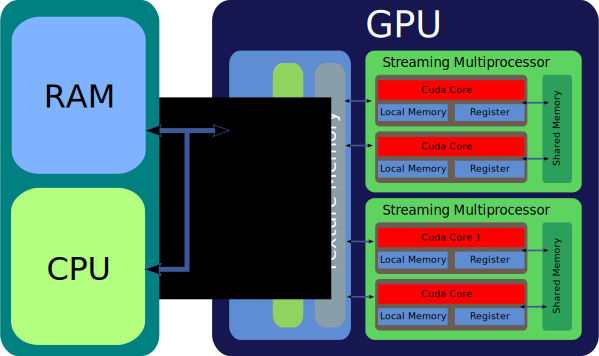
\includegraphics[width=0.8\textwidth]{gfx/cuda/gpu.png}\label{fig:gpu_arch}
  \caption{Speicherlayout einer Nvidia-GPU}
\end{figure}

-bild
-speicher bereiche
-grid layout function call
-threadidx etc

\section{Algorithmus}
-oder so ?
-erläuterung  implementierung
-speicherverwaltung

\section{Optimierung}
- coalesceded
- bank conflicts?
- teilvolumen nicht rechnen

\section{Validierung}
- beispiel rayleigh benard system
- masa
- vgl o2 vs o4 masa cube
- bifurcation


\newpage



\chapter{Immersed Boundary Methods for No-Slip Walls}
\section{Overview of Immersed Boundary Methods}

\begin{figure}[!bp]
  \centering
  \subfloat[cartesian grid]{\includegraphics[width=0.4\textwidth]{gfx/immersed_boundary_methods/general_partition_triangle.jpg}\label{fig:grid_f1}}
  \hfil
  \subfloat[unstructured body-fitted grid]{\includegraphics[width=0.4\textwidth]{gfx/immersed_boundary_methods/general_partition_triangle.jpg}\label{fig:grid_f2}}
  \caption{Different types of numerical grids}
\end{figure}

For many fluid problems it is mandatory to solve the equations of motion with respect to complex-shaped geometries \.
The algorithm introduced in section () is not yet suitable for such a scenario.
For instance the simulation inside a spheric geometry is impossible, since the boundaries
do not coincide with the implemented cartesian grid. Nevertheless there exist different approaches to overcome this problem,
which shall be introduced here. \\
The common approach to extend the algorithm would be to use a body-fitted mesh (see figure \ref{fig:grid_f1}),
different advantages and disadvantages arise with this kind of implementation (see \citep{Mittal2005}).
One benefit is a much simpler deployment of the desired boundary condition, due to the overlap of the grid with domain border.
Furthermore a higher accuracy can be achieved \citep{Gornak2013}.
However, using an unstructered grid generates plenty of computational overhead, during and before the execution of a simulation.
The generation of the grid is very complicated in contrast to using a cartesian grid, this can be even more complicated when
considering moving boundaries.
Also solving the finite differenc schemes on a curvilinear coordinate system, leads to more calculations on a single grid point.
The last important aspect is the implementation on the gpu.
Like discussed in section () it is more efficient to use homogenous storage and calculation pattern on a CUDA-device,
the use of unstructured data makes this very difficult.
Altough some attempts exists to solve these difficulties (see i.e. PAP), it is still uncertain if the obtained performance loss would be acceptable.\\
A set of alternative methods, to resolve the problems described above, are so called Immersed Boundary Methods.
The term was first mentioned in (PESKIN 1972), for the simulation of blood flow through a heartvale, but has since then been used for a variety of
methods (MITTAL).  All of them have the idea in common to perform the simulations on a cartesian grid which does not conform to the domain boundary.
To satisfy the desired boundary conditions additional terms are introduced into the equations of motion.
In general one can distinguish between contiuous forcing methods and direct forcing methods.
Continious forcing methods try to mimic the boundary using a localized force which acts on the boundary,
since the surface is tracked by lagrangian points this methods can be well suited for moving boundaries (MITTAL).
One common problem is that continous forcing can arise to stability problem and numerical oscillations in numericial stiff problem (SOURCE).
The direct forcing approach tries to satisfies the boundary condition, by imposing it directly to points near the fluid surface for example
trough an interpolaltion procedure.
Some of the major drawbacks using the IBM is the loss in  spatial accuracy at the boundary, therefore it can be necessary to use a higher grid resolution
compared to a body-fitted mesh.  Futhermore the non-conforming (?) boundaries are more difficult implement.
The benefits of these methods is the use of a cartesian grid, which is much more suited for a gpu-based implementation (see section X).
As a result the overall performance will probably be in the same order as the original algorithm.
In the thesis the Implementation of different Immersed Boundary Methods is seperated into three chapters depending on the boundary condition and application.
This chapter beginns with Implementation of NoSlip-Walls which are the easisest to implement.
The term Immersed Boundary Method is vaguely defined in literature, in this thesis we refer to it with all methods introduced in the following three chapters.

\newpage

\section{IBM-Methods}
\section{Volume Penalization}

%Die Volume-Penalization Methode ermöglicht es, durch einen Kraftterm der auf die einzelnen Fluidzellen wirkt, mit wenig Aufwand Noslip-Ränder zu implementieren.
%Das Verfahren wurde in mehreren Publikationen z.B. [bla] erfolgreich verwendet, eine mathematisch exaktere Abhandlung lässt sich z.B. in [bla2] finden.
%
%\begin{wrapfigure}{r}{0.5\textwidth}
%  \begin{center}
%  \includegraphics[width=0.5\textwidth]{gfx/immersed_boundary_methods/mask.png}\label{fig:mask_vp}
%  \includegraphics[width=0.5\textwidth]{gfx/immersed_boundary_methods/mask.png}\label{fig:mask_vp}
%  \end{center}
%  \caption{Maskierungsfunktion $H(x,y,z=const.) = x^2 + y^2 < c$ für einen Zylinder. }
%\end{wrapfigure}
%
%Das Volumen wird zunächst in einen Fluidbereich und einen festen Wandbereich, wie in Abb.1 dargestellt, unterteilt. Für die Differenzierung der Bereiche während der Simulation wird  eine Maskierungsfunktion
%\begin{align}
%H(x, y, z) = \begin{cases}
%                    0, & \text{für } \vec{x}(x,y,z) \in Fluid, \\
%                    1, & \text{sonst}.
%             \end{cases}
%\end{align}
%verwendet. Als zusätzlicher Kraftterm wird nun eine exponentielle Dämpfung eingeführt die nur auf den Wandbereich des Volumens wirkt.
%\begin{align}
%\vec{f} = \frac{H(x, y, z)}{\nu}(\vec{v} - \vec{v_0})
%\end{align}
%Bei $\vec{v_0}$ handelt es sich um die gewünschte Randbedingung, der Kraftterm ist also proportional zur Auslenkung $\vec{v}$ eines Punktes vom gewünschten Ruhezustand.
%Die Antwort des Kraftterms wird durch die Dämpfungrate $\nu$ reguliert. Je kleiner $\nu$ desto stärker ist die Dämpfungsrate, allerdings kann der Term
%nicht beliebig klein gesetzt werden da die Stabilität für $\nu < dt$ nicht mehr gewährleistet ist [source].
%Da für die Lösung der der Geschwindingskeitsfelder mit der Methode der künstliche Kompressibilität  bereits ein sehr kleiner Zeitschritt verwendet wird (s.Abb. X)
%kann im Vergleich zu anderen Verfahren wie z.B. (pseudo-spektrale) eine relativ starke Dämpfungsrate verwendet werden.
%
%\subsubsection{Validierung mit MASA}
%-validierung mit masa für alle verfahren oben.. cube /evtl zylinder?
%-vegl. und argumentation ränder ehh auf null.
%-ein beispiel mit vol.pen.
%
%\subsubsection{Validierung : planare Poiseuille Strömung}
%Es stellt sich die Frage in welcher Größenordnung die Dämpfungskonstante $\nu$ der Volume Penalization methode liegen muss, um einen möglichst kleinen
%Fehler zu gewährleisten. Ein einfacher Testfall der sich hierfür betrachen lässt ist eine einfache planare poiseuille strömung, diese ist schematisch in Abb. (x). dargestellt.
%\paragraph*{Theoretische Beschreibung}\mbox{}\\
%Wir betrachten eine laminare Strömung in x-Richtung die durch einen Druckgefälle $f=-\frac{\partial p}{\partial x}$ angetrieben wird.
%Für die x- und y-Richtung werden periodische Randbedingungen angenommen. In z-Richtung wird das Volumen durch zwei Ebenen bei $h_1$ und $h_2$ begrenzt,
%es gilt $ \vec{v}(z=h_1) = \vec{v}(z=h_2) = 0$.
%Im stationären Fall lässt sich  die Bewegungsgleichung dann  auf eine Dimension reduzieren, es gilt:
%
%\begin{align}
%\frac{\partial v_x}{\partial t} &= - \frac{\partial p}{\partial x} + D \frac{\partial^2 v_x}{\partial z^2} = 0 \\
%\Rightarrow v_x &= \frac{1}{2D}\frac{\partial p}{\partial x}z^2 + zc_1 + c_2\\
%\end{align}
%
%Mit $\vec{v}(h_1) = \vec{v}(h_2) = 0$ und $A:=\frac{1}{2D}\frac{\partial p}{\partial x}$ ergibt sich:
%\begin{align}
%c_1 &= A\frac{h_1^2 -h_2^2}{h_2 - h_1} = -A(h_1+h_2)\\
%c_2 &= A(h_1(h_1 + h_2) - h_1^2) = Ah_1h_2\\
%\Rightarrow v_x &= A(z^2 - z(h_1 + h_2) + h_1h_2)
%\end{align}
%Da die Strömung in der Kanalmitte am stärksten ist gilt zudem:
%\begin{align}
%z_{max} &= \frac{h_1+h_2}{2}\Rightarrow v_{max} = A\left(h_1h_2 - \frac{(h_1 + h_2)^2}{4}\right)
%\end{align}
%Für die Strömung lässt sich die Reynoldszahl dann gemäß $Re \propto \frac{v_{max}}{D}$  bestimmen.
%\begin{figure}[!hbtp]
%  \centering
%  \includegraphics[width=0.9\textwidth]{gfx/immersed_boundary_methods/vp_flow.png}\label{fig:vp_flow}
%  \caption{Geschwindigkeistprofile im Kanal bei Variation der Dämpfungskonstante $\nu$ und Reynoldszahl $Re=500$.}
%\end{figure}
%
%\paragraph*{Setup}\mbox{}\\
%Um die Abhängigkeit des Fehlers von der Dämpfungskonstante zu betrachten wurde ein Kanal mit $l_x=1$, $l_y=1$ und $l_z=2$ sowie $h_1=0.25$, $h_2=0.75$.
%betrachtet. Die Maskierungsfunction ergibt sich damit gemäß $H(z) = (z>h1) \wedge (z<h2)$.
%Für die Reynoldszahl wurden Werte im Intervall $Re \in [100, 500]$ verwendet, die Dämpfungskonstante wurde zwischen $\nu \in [1e-5, 0.1]$ variert, während der Zeitschritt mit $dt =1e-5$ konstant gehalten wurde. Die genauen Angaben für alle Parameter sind in (Anhang Tab.X) zu finden.
%
%\paragraph*{Ergebnisse}\mbox{}\\
%Zunächst ist in Abb. \ref{fig:vp_flow} das Geschwindigkeitsprofil der Strömung für $Re=500$ exemplarisch dargstellt. Es lässt sich bereits qualitativ sehr gut erkennen, dass für eine
%starke Dämfung die Kanalströmung an den Grenzen $h_1$ und $h_2$ verschwindet und gut mit der dem theoretischen Profil übereinstimmt.
%Bei einem Verringern der Dämpfungrate entwickelt sich im Rand ein Geschwindigkeitsprofil.
%Um sicherzustellen dass sich das Profil vollständig entwickelt wurde die Simulation bis zu dem Zeitpunkt fortgegeführt
% in welchem die kinetische Energie des Systems einen stationären Wert erreicht. Anschließend wurde der absolute und relative Fehler mit Formel (X) berechnet,
%dabei wurde das theoretische Profil gemäß () verwendet. Die Ergebnisse sind in Abbildung \ref{fig:vp_error} dargestellt.
%
%\begin{figure}[!bp]
%  \centering
%  \includegraphics[width=1.0\textwidth]{gfx/immersed_boundary_methods/vp_error.png}\label{fig:vp_error}
%  \caption{Absoluter und relativer Fehler in Abhängigkeit von Dämpfungskonsante $\nu$ und Reynoldszahl $Re$.}
%\end{figure}
%
%Bei beiden Fehler lässt sich ein Abfall bis $\nu=1e-4$ erkennen, anschließend kommt es zu einem minimalen Anstieg.
%Betrachtet man den absoluten Fehler, so fällt auf das im Bereich $\nu>5\cdot10^{-3}$, mit steigender Reynoldszahl, der Fehler zunimmt.
%Dies entspricht zunächst der Erwartung, da das Geschwindigkeitsprofil mit steigender Reynoldszahl stärker an der Wand zerrt.
%Allerdings kommt es im Bereich $\nu \in [1e-3 - 1e-2]$ zu einem umgekehrten Verhalten, der Fehler nimmt mit der Reynoldszahl ab,
%Du Ursache hierfür liess sich nicht eindeutig klären.
%Für den relativen Fehler lässt sich ein Abfall mit steigender Reynoldszahl beobachten. Da $\vec{f} \propto (\vec{v}-\vec{v_0})  \propto Re$ wird der Reibunsterm
%proportional zur Reynoldszahl skaliert. Der Fehler durch den Rand ändert sich, im Vergleich zum Geschwindigskeitsprofil kaum, wodurch der Abfall zustande kommt.
%Der relative Fehler fällt bei $\nu=1e-4=10\Delta t$ auf unter 1\%, wodurch dieser Wert als geeignet angesehen werden kann für zukünftige Simulationen mit der Volume-Penalization Methode.
%
%-todo: fluktuation im rand
%
%
%\subsection{Direct Forcing Methode}
%Während die Volume Penalization Methode die Geschwindigkeit ausserhalb des Volumens nicht vollständig auf Null setzt,
% kann dies durch eine implizite Berechnung des Dämpfungsterm erreichtwerden. Es stellt sich heraus das dieser Ansatz equivalent
%  zu der Direct Forcing Methode ist, die erstmals von [] verwendet und in [] beschrieben wird.
%Betrachten wir zunächst den diskretisierten Zeitschritt
%\begin{align}
%    \frac{\vec{u}^{n+1} -\vec{u}^n}{\Delta t} = \mathscr{L} + \vec{f}\\
%\end{align}
%wobei $\mathscr{L}$ den diskretiesierten Operatoren der PDE entspricht.
%Für einen Punkt auf dem Rand des Volumens soll nun die Randbedingung $\vec{u}^{n+1} = \vec{u}_0$ eingehalten werden.
%Mit Formel () folgt
%\begin{align}
%    \frac{\vec{u}_0 -\vec{u}^n}{\Delta t} = \mathscr{L} + \vec{f} \Rightarrow \vec{f} = \frac{\vec{u}_0 -\vec{u}^n}{\Delta t\cdot \mathscr{L}}\\
%\end{align}
%Mit der Annahme dass der Rand mit dem numerischen Gitter übereinstimmt ist es nicht nötig den Kraftterm zur berechnen, stattdessen lässt sich der
%Schritt vereinfachen in dem der Randwert nach  jedem Zeitschritt direkt auf die gewünschte Randbedingung gesetzt wird. Durch die
%implizite Behandlung kommt es zu keiner weiter Stabilitätsbedingung.
%Analog zur Volume-Penalization Methode wurde eine Serie von Simulationen für eine planare Poiseuille-Strömung durchgeführt.
%Das Setup enstpricht dem gleichen wie in Abschnitt (X), lediglich das Verfahren wurde entsprechend angepasst und es wurden finite Differenzen Verfahren zweiter und
%vierter Ordnung getestet.
%In Abbildung () ist der relative Fehler, im Vergleich zur Volume Penalization  Methode mit $\nu=1e-4$ dargestellt.
%Für das Verfahren vierter Ordnung liegt der Fehler im Bereich von 1\% und ist im Mittel doppelt so groß wie für die Volume-Penalization Methode.
%Der Fehler für das Verfahren zweiter Ordnung verschwindet hingegen nahezu.
%Das Verhalten lässt sich durch die Verwendung unterschliedlicher Schablonen, wie in Abb() dargestellt,  der finiten differenzen Verfahren erklären.
%Während das Verfahren zweiter Ordnung nur den Randpunkt sieht, liegt bei der vierten Ordnung ein Punkt innerhalb des Randes.
%Da auch dieser Wert auf Null gesetzt wird, kommt es zu einem fehler in der Berechnung von $\nabla u$.
%
%\begin{figure}[!tpb]
%  \centering
%  \includegraphics[width=0.6\textwidth]{gfx/immersed_boundary_methods/dfo2o4.png}\label{fig:df_o2o4}
%  \caption{bla}
%\end{figure}
%
%-Zeitserie
%
%-einleitung gekrümmte geometrien
%
%\subsection{Direct Forcing mit Volume Fraction}
%-paper quote formeln
%-implementierung beispiel
%
%\section{Direct Forcing mit Interpolation}
%-paper quote formeln
%-implementierung beispiel
%
%\section{Methoden-Vergleich und numerische Validierung}
%In diesem Abschnitt sollen die verschiedenen Methoden über numerische Testfälle validiert und miteinnander
%verglichen werden.
%
%
%\subsubsection{Poiseuille Strömung im Zylinder}
%
%\subsubsection{Zusammenfassung}
%
%
%\subsection{No-Flux-Boundaries}
%
%\subsubsection{'Variable Konduktivität'}












\chapter{IBM2}
\clearpage
\section{Validation}

%This part of the thesis the thesis deals with the numerical validation of the immersed
%boundary methods
%In the first part of the chapter an introduction to different test cases
%will be given. Three different test problems were chosen.
%The flow between to planes, also known as Planar Poiseuille flow, the flow in a Pipe, referred to as Hagen-Poiseuille flow and the flow
%between two rotating cylinders, know as the Taylor-Couette system.
%In the second part of the chapter the result for the different test cases will be presented and discussed.
%In the first part of the chapter an introduction to different test cases
%will be given.
This section presents the numerical validation of the immersed boundary methods.
The objective of the validation is to determine the numerical accuracy and
the numerical stability for each method.
Furthermore it is important to test if conservation laws, in particular the conservation of mass,
are fulfilled.
For the validation three different test problems were chosen.
The flow between to planes, also known as Planar Poiseuille flow, the flow in a Pipe, referred to as Hagen-Poiseuille flow and the flow
between two rotating cylinders, know as the Taylor-Couette system.

\paragraph{Conventions}\mbox{}\\

In this section the following abbreviations will be used

\begin{multicols}{2}
\begin{description}
    \item[VP]{Volume-Penalization Method}
    \item[DF]{Direct Forcing Method}
    \item[IP]{Interpolation Method}
    \item[VF]{Volume-Fraction Extension}
    \item[o2]{Finite Difference Schemes of 2nd order}
    \item[o4]{Finite Difference Schemes of 4th order}
\end{description}
\end{multicols}

For example, DF-VF-o2 method, refers to the Direct-Forcing method, extended with the Volume-Fraction
method and the use of 2nd order finite difference schemes.

\paragraph{Grid Convergence Studys}\mbox{}\\

For the validation multiple grid convergence studys were performed.
The concept of a grid convergence study is to vary the grid resolution of the numerical domain and
calculate the error of the simulation with respect to an assumed theoretical solution.
The relative error $\epsilon$ is computed by the relative $l_2$-norm

\begin{align}
    \epsilon = \frac{\int \dif V \left(a^{\text{th}} - a^{\text{num}}\right)^2}{\int \dif V \left( a^{\text{th}} \right)^2}
     = \frac{\sum_{i,j,k}^{N_x, N_y, N_z}
      \left(a^{\text{th}}_{i,j,k}  - a^{\text{num}}_{i, j, k}  \right)^2}
     {\sum_{i,j,k}^{N_x, N_y, N_z} \left( a^{\text{th}}_{i,j,k} \right)^2}
 \end{align}

where $a^{\text{th}}$ corresponds to the theoretical and $a^{\text{num}}$ to the numerical solution.
The numerical error is usually given by a power law of the form $\epsilon = N^\lambda$, i.e for a finite difference scheme of 2nd order
this is the truncation error given by the remaining terms  of the taylor expansion.
For an evaluation of the error convergence the results of the grid convergence study are, if possible, linear fitted in the log-log space, to obtain the
convergence rate $\lambda$.




%In general it is necessary to obtain a good evaluation of the numerical truncation error,
% the numerical stability over longer periods of time
%and Grid convergence studys against theoretical and high-resolution numerical solutions
%will be performed and compared for the different IBMs.
%In order to ensure a correct numerical behavior of the introduced methods, a
%Multiple examples from simple to more complex test cases are introduced in this section.
\clearpage

\subsection{Laminar Poiseuille-Flow}

\begin{figure}[!bp]
  \begin{minipage}[c]{0.6\textwidth}
      \centering
        \resizebox{0.9 \textwidth}{!}{
       \import{gfx/immersed_boundary/poiseuille_flow//}{setup.pdf_tex}
      }
  \end{minipage}
  \begin{minipage}[c]{0.3\textwidth}
      \caption{Setup of the Poiseuille-flow channel.
      \label{validation:setup_pf}
      }
  \end{minipage}
\end{figure}

The first test case is the laminar poiseuille-flow. The theoretical setup is presented in Fig. \ref{validation:setup_pf}.
It consist of two infinite extending  planes at $z=h_1$ and $z=h_2$, which are oriented
parallel to the xy-plane, at a distance $\Delta h = h_2 - h_1$.
Numerically this is realized by using periodic boundaries in xy-direction and
No-Slip boundaries in the z-direction.

The velocity profile is a result from a predefined spatial constant pressure gradient $\nicefrac{\partial p}{\partial x}$
 in x-direction, that is added into the Navier-Stokes equation.
The steady state for the non-dimensional equations is given by \citep{}
\begin{align}
    \label{vali:pflow_navstok}
    \frac{\partial v_x}{\partial t} &= - \frac{\partial p}{\partial x}
     + \frac{1}{Re} \frac{\partial^2 v_x}{\partial z^2} = 0
\end{align}

with the Reynolds-number defined as $Re = \nicefrac{V_{m}\Delta h}{\nu}$.
For this system the non-dimenzionalization is given by the scales
    $r^* = \nicefrac{r}{\Delta h}$, $v^*=\nicefrac{V_(\text{m})}{\Delta h}$,
    $t^* = \nicefrac{V_{\text{m}}}{\Delta h}$ and $p^* = p \rho V_{\text{max}}^2$.

The velocity $V_m$ is defined as $\max(v_x(z))$.
An integration of Eq. \ref{vali:pflow_navstok} gives
\begin{align}
v_z &= \frac{1}{2}\frac{\partial p}{\partial x}z^2 + zc_1 + c_2
\end{align}

Using the NoSlip-boundary condition $v_x(h_1) = v_x(h_2) = 0$ and furthermore by defining
$A:=\frac{1}{2}\frac{\partial p}{\partial x} Re$ one obtains the additional conditions

\begin{align}
c_1 &= A\frac{h_1^2 -h_2^2}{h_2 - h_1} = -A(h_1+h_2)\\
c_2 &= A(h_1(h_1 + h_2) - h_1^2) = Ah_1h_2
\end{align}

The velocity is than given by the quadratic function
\begin{align}
\label{vali:pflow_theosol}
v_x &= A(z^2 - z(h_1 + h_2) + h_1h_2)
\end{align}

The maximum velocity and position are given by
\begin{align}
z_{max} &= \frac{h_1+h_2}{2} \wedge v_{max} = A\left(h_1h_2 - \frac{(h_1 + h_2)^2}{4}\right)
\end{align}

$V_{m}$ has to be 1 by the definition of the non-dimensionalzation. This gives
\begin{align}
\frac{\partial p}{\partial x} &= \frac{2}{Re}\frac{1}{\left(h_1h_2 - \frac{(h_1+h_2)^2}{4} \right)}
\end{align}
as a necessary condition for the pressure gradient.

\subsection{Simulations}

The Poiseuille-flow test case is used in particular as a first validation
for the Volume-Penalization and Direct-Forcing methods.

\subsubsection{Test of the Default Setup}

The purpose of the first simulation is the test of the default
implementation of the algorithm, without the use of immersed boundaries.
For this test case this is still possible since the geometry is non-curved
and parallel to the cartesian grid.
A grid convergence test was performed with the main simulation parameters given by

\begin{center}
\vspace*{0.7ex}
\begin{tabular}{c|c|c|c|c|c|c }
 $ N  $                   & $\Delta t$ & $\Delta x$            & $\Rey$  & $c^2$   & $l_x, l_y, l_z$ & $T_{end}$\\
\hline
 $[8, 256], \Delta N = 8 $& $10^{-4}$ & $\nicefrac{1}{N - 1}$ & 500     & $500$   & (1, 1, 1)       & 10\\
\end{tabular}
\vspace*{0.7ex}
\end{center}

The simulations were performed for finite difference schemes of 2nd and 4th order.

\subsubsection{Test of the Volume Penalization Method}

%With the given theoretical solution, the next objective is the comparison
%to the default implementation, the volume penalization method and the direct forcing method.
%Since we have a flow parallel to the grid  it does not make sence to compare it to the interpolation methods
%For the comparision with a theoretical solution it is necessary to ensure that
% the surface grid points match with the total height $h$ of the channel.

For the immersed boundary methdos the upper- and lower boundaries of the channel are realized by the masking function.
\begin{align}
H(x, y, z) = \begin{cases}
                    0, & \text{for \  }  h_1 \leq z \leq h_2 \\
                    1, & \text{else}.
             \end{cases}
\end{align}

For the volume penalization method we furthermore obtain a
The non-dimensionalized damping force  given by

\begin{align}
    \vec{f} = \frac{H}{J}v
\end{align}

where $J = \nicefrac{V_{m}}{\eta}$.
A first test is to investigate the error of the velocity profile, with a variation of the Reynolds-number and the damping rate $J$.
The total simulation domain is set to the height $l_z=2$ with $h_1=0.25$ and $h_2=0.75$.
A simulation series was performed with the main simulation parameters given by


\begin{center}
\vspace*{0.7ex}
\begin{tabular}{c|c|c|c|c|c|c|c }
 $ \Rey  $                      & $J$ &  $\Delta t$ & $\Delta x$            & $\Rey$  & $c^2$   & $l_x, l_y, l_z$ & $T_{end}$\\
\hline
 $[100, 500], \Delta \Rey = 25 $& $[10^{-5}, 5\cdot10^{-1}]  $ &  $10^{-4}$ & $\nicefrac{1}{N - 1}$ & 500     & $500$   & (1, 2, 0.25)  & 10\\
\end{tabular}
\vspace*{0.7ex}
\end{center}

The damping force was divided by 2 or 5 for n times(EXPLAIN).
To make sure that the channel width is equal to $\Delta h = 1$, the total height was set to $l_z\approx2.01587$.
This ensures that the grid points overlap exactly with the masking function at $h_1=0.25$ and $h_2=0.75$.
The simulations were performed for the 2nd order method. (O4 EXPLAIN)

As a second test a grid convergence study was carried out, with a constant Reynolds number and $J \in [1-23]$.
The resolution was varied between $N\in [4, 400]$ with $\Delta N = 4$, 2nd and 4th order schemes were tested.

\begin{center}
\vspace*{0.7ex}
\begin{tabular}{c|c|c|c|c|c|c|c }
 $ \Rey  $                      & $J$ &  $\Delta t$ & $\Delta x$            & $\Rey$  & $c^2$   & $l_x, l_y, l_z$ & $T_{end}$\\
\hline
 $[100, 500], \Delta \Rey = 25 $& $[10^{-5}, 5\cdot10^{-1}]  $ &  $10^{-4}$ & $\nicefrac{1}{N - 1}$ & 500     & $500$   & (1, 2, 0.25)  & 10\\
\end{tabular}
\vspace*{0.7ex}
\end{center}

\subsubsection{Test of the Direct Forcing Method}

Since the direct forcing method does not depend on a damping parameter it is sufficient enough
to carry out a grid convergence study
The simulation parameter are given by

\begin{center}
\vspace*{0.7ex}
\begin{tabular}{c|c|c|c|c|c|c|c }
 $ \Rey  $                      & $J$ &  $\Delta t$ & $\Delta x$            & $\Rey$  & $c^2$   & $l_x, l_y, l_z$ & $T_{end}$\\
\hline
 $[100, 500], \Delta \Rey = 25 $& $[10^{-5}, 5\cdot10^{-1}]  $ &  $10^{-4}$ & $\nicefrac{1}{N - 1}$ & 500     & $500$   & (1, 2, 0.25)  & 10\\
\end{tabular}
\vspace*{0.7ex}
\end{center}

2nd and 4th order finite difference schemes were tested.

\clearpage

\subsection{Results}
\subsubsection{Default seutp}

The results of the grid convergence study are shown in Fig. \ref{fig:ema1}.
The double logarithmic axis shows the dependency of the computed relative $l_2$-error norm
with respect to the grid resolution.

On this scale, the 4th order finite difference scheme has a linear decreasing error.
For the smallest resolution $N=8$ the error is of order $10^{-3}$,
in contrast to the highest resolution $N=256$ with an error of order $10^{-6}$
A convergence rate of the error  was computed by linear interpolation in the log-log space,
the results is about -2.257.
Hence, it can be said that the accuracy of the method is of 2nd order for this test case,
which is is in contradiction with the theory.

The error of the 2nd order finite difference scheme is of the order $10^{-8}$.
The value is approximately constant and not depend of the grid resolution.

\begin{figure}[!bp]
    \centering
    \includegraphics{gfx/immersed_boundary/poiseuille_flow/1_default/relative_l2error.pdf}
    \caption{Relative $l_2$-error for 2nd and 4th order finite difference schemes of the default algorithm without the use of an immersed boundary.\label{fig:ema1}}
\end{figure}

\clearpage


\subsubsection{Test of the Volume Penalization Method}

The first simulation was  a parameter study with variable Reynolds number $Re$ and damping rate $J$.
A first impression of the influence of the damping rate $J$ , is given by the velocity profiles of the numerical solution.
This is exemplarily shown in Fig. \ref{fig:vp_flow}, for variable $J$ and a constant reynolds number $Re=500$.
It can be noted that with an decrease of $J$, the numerical solution converges against the theoretical one.

\begin{figure}[!b]
  \centering
  \includegraphics{gfx/immersed_boundary/poiseuille_flow/2_vp/vp_profile.pdf}  \caption{\label{fig:vp_flow}
    Velocity profile of the numerical solution with variable $J$ and $\Rey = 500$.}
\end{figure}

Furthermore it can be seen that the quadratic part of the velocity profile,
inside of the fluid domain ($0.5\leq z \leq 1.5$), is independent of the damping constant $J$.
Merely a slight offset at the boundaries creates a constant shift of the velocity profile.
In the masked area of the volume a decrease in velocity is visible which could  eventually be described by an
exponential law.

For an error estimation, the relative $l_2$-error was computed.
The results for the 2nd order scheme are shown in Fig. \ref{fig:vp_error}.
\begin{figure}[!b]
  \centering
  \includegraphics{gfx/immersed_boundary/poiseuille_flow/2_vp/vp_error.pdf}  \caption{\label{fig:vp_error}
    Relative $l_2$-error for variable damping rate $\nu$ and Reynolds number $Re$.}
  \centering
  \includegraphics{gfx/immersed_boundary/poiseuille_flow/2_vp/vp_convergence.pdf}
  \caption{\label{fig:vp_conv}
      Relative $l_2$ error for variable damping rate $J$, for 2nd (blue) and 4th (red) order finite difference schemes.}
\end{figure}

On the left side of the plot the relative error is plotted against the damping rate, the reynolds number is
varied over a color scale. On the right side both variables are switched.

A decrease in the damping rate $J$ results in an decrease of the error about four orders, from $10^{-1}$ to $10^{-5}$.
With a change of the Reynolds number from $500$ down to $100$ the error decrease about one order.
It can be noticed that with an decrease of $\Rey$ or $J$ the error decreases linear in the log-log space.
For a small damping ($J>10^{-3}$) a breakdown of the linear relation can be observed.
This is an error resulting from the numerical setup.
\clearpage

The damping in the masking area is so weak that the flow reaches the  boundaries of the numerical domain.
This is not the case for $J<1e-3$ since the velocity profile is zero before it reaches the boundaries.\\
A linear fit in the log-log space gives a  decay rate of about $1.106$ for  $J$ and about $-1.223$ for $\Rey$.

The second part of the test was a grid convergence study with a constant Reynolds number, variable $J$ and grid resolution $N$.
The results are shown in Fig. \ref{fig:ema1}.

It can be noticed that a decrease in $\nu$ creates a shift in the error profile to overall smaller values.
However it is also noticable that the error of the 2nd order scheme, increases together with the resolution.
Even less understandable is the error function for the 4th order scheme.
With increasing resolution  a decrease into a minimum, followed by an increase can be observed.

The position of minimum is shifted to the right with an decrease of $J$.
For a constant $J>10^{-4}$ it is visible that the error for both methods converges against a
constant error  with an increase in the resolution.

\subsubsection{Direct Forcing Method}

The results of the grid convergence study are similat to the results of the default implementation,
except the fourth order scheme has a larger error.
A plot of the relative $l_2$-error can be found in the Appendix  in Fig. \ref{fig:ema1}.
The 4th order finite difference schemes has a linear decreasing error in the log-log space..
For the smallest resolution $N=8$ the error is of order $10^{-2}$,
in contrast to the highest resolution $N=256$, with an error of order $10^{-4}$
The convergence rate is about $1.267$
Hence, it can be said that the accuracy of the method is of 1st order for this test case.
The error of the second order finite difference scheme is of the order $10^{-8}$.
The value is approximately constant and not depend of the grid resolution.

\clearpage

\subsection{Discussion}
\subsubsection{Default setup}


The constant error of the 2nd order scheme is due to the lack of complexity of the test case.
As the theoretical solution for the test case is a polynom of 2nd order,
no higher order terms will occur in the numerical solution, hence the
2nd order scheme is capable of a perfect approximation, independent of the
grid resolution. The remaining error terms, wich  are of the order $10e^{-8}$,
occur due to the round off error of the single precision floating-point format.

The convergence of the fourth order scheme, which is of 2nd order in this test case,
reveals that an error exists in the default implementation of the NoSlip boundaries.
An explanation can be given with a comparison to the theoretical solution.
The 2nd derivative is given by

\begin{align}
    \pdn[^2 v_x]{x^2} = \frac{1}{\Rey}\pdn[p]{x} := C\in\mathbb{R}
\end{align}

The default algorithm uses a mirroring method on the boundaries of the fluid domain (see Sec. \ref{XXX}), for the No-Slip boundaries.
Let $C_b$ be the derivative in the immersed boundary, it follows that $C_b = - C$, as a result of the mirroring.
Therefore a discontinuity of the 2nd derivative is created at the boundaries.
When using the 2nd order method the 3-Point stencil evaluates to the correct value.
The 5-Point stencil of the 4th order scheme evaluates to a false value, since it uses one point behind the boundary.
As a result the discontinuity creates an error in the 4th order scheme.

\subsubsection{Test of the Volume Penalization Method}

The offset on the boundaries arises since the Volume-Penaliztation method cannot fullfill the exact boundarie conditions.
For the steady state a force equillibrium at the boundaries is given by the pressure gradient, the laplace operator and the damping force

\begin{align}
\label{valid:steady_state_pflow}
 J v_x &=  \frac{1}{\Rey}\frac{\partial^2 v_x}{\partial z^2} -\pdn[p]{x}
\end{align}

which results in a constant offset $v_x(h_1) = v_x(h_2) =: C\in\mathbb{R}$.
The simultaneous decrease of the $l_2$-error with $J$ is as expected.
However it is counterintuitive that the $l_2$-error decreases with an increase of the Reynolds number.
An explanation for this is, that the viscous force and the pressure gradient are proportional to $\nicefrac{1}{\Rey}$.
With an increase of the Reynolds number the steady state in Eq. \ref{valid:steady_state_pflow} is shifted.
The result is a smaller offset on the sides and and overall smaller error.

\begin{figure}[!tp]%
    \centering
    \subfloat[label 1]{{
    \label{fig:example_a}%
      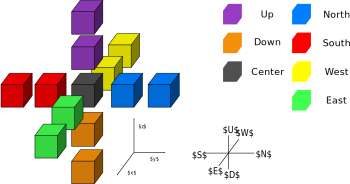
\includegraphics{gfx/immersed_boundary/poiseuille_flow/discussion/stencil.pdf}
            }}%
    \qquad
    \subfloat[label 2]{{
    \label{fig:example_b}%
      \includegraphics{gfx/immersed_boundary/poiseuille_flow/discussion/profile.pdf}
        }}%

\end{figure}

The grid convergency study with a constant Reynolds number and variable damping rate, generates an error
which increases simulatenous with the grid resolution.
An explanation for this behavior can by given by revising the theoretical solution
and the finite difference stencils at the immersed boundary.

The error for both method does not converge towards zero, which means there has to be some discrepancy to the theoretical solution given by
Eq. \ref{vali:pflow_theosol}.
For a constant $J$ there is an offset $C$ to the theoretical solution,
which is given by the equillibrium accord to Eq.  \ref{valid:steady_state_pflow}.
This means that the theoretical solution which was assumed in the first place, is wrong for the Volume-Penalization method.
An additional offset in the flow, which is dependent of the damping rate $J$ has to be considered.
For a low resolution, the profile of the 2nd order method is closer to the assumed theoretical, which results in a smaller
error. With an increase to a higher resolution the error with respect to the real solution decreases.

An explanation for the convergence of the 4th order can be given by furthermore considering the descrization error at the immersed boundaries.
Fig. \ref{fig:example_a} shows exemplary the velocity profile near to the immersed boundary, for the Volume-Penalization method of 2nd and 4th order
at a resolution of $N=100$.
It can be seen that the velocity profile for the 4th order method, is slighty negative.
The reason for this is the use of a 5-Point stencil for the discretization.
The stencil reaches over the immersed boundary which results in a wrong computation of the laplacian.
An explanation for the 4th order convergence is given by the velocity profiles for different resolutions,
as shown schematically in Fig. \label{fig:example_b}.
\footnote{The difference in the computed velocity profiles is barely visible, therefore an exaggerated version is used.}
The velocity profiles for three different resolutions are considered for a constant $J$,
the minimum of the error shall be defined as $N_{min}$.
Due to the negative velocity at the boundary the first profile $N<N_{min}$ lies below the theoretical assumed.
The second profile is at $N=N_{min}$. The error at the boundary is smaller due to the increase of the resolution.
The profile overlaps best with the theoretical solution resulting in the minimal error.
With a further increase of the resolution  $N>N_{min}$ the velocity profile drifts away from the theoretical solution,
the error increases.  Finally the method converges towards the same solution as the 2nd order scheme.


\subsubsection{Direct Forcing Method}

The results for the direct forcing method show that d


-We can see o4 not working reason is the same as we can se in Fig. n) , the laplacian is wrong caclulated at the point B.
As a results an error is induced at the boundaries of the domain.
The 2nd order scheme works perfectly as we compare it to the default implementation.


\section{Blub}
\subsection{Hagen-Poiseuille Flow}

In the previous test case the channel walls were aligned parallel to the simulation grid. Hence, no further interpolation procedures
are necessary to mimic the exact boundaries.
In order to test the accuracy of the Volume-Fraction and the Interpolation method, a test case with a curved geometry is necessary.
Furthermore this gives the possibility to investigate the error of non-interpolating methods on curved surfaces.
A simple adaption of the planar Poiseuille flow, is the laminar flow through a pipe, also referred to as Hagen-Poiseuille flow \citep{tritton88}.
The setup of the fluid domain is schematically shown in Fig. \ref{validation:setup_hpflow}.

It consist of a circular pipe with the radius $r$, which extends infinitely, parallel to the $x$ axis.
This is realized by using periodic boundaries in $x$-direction.
The center of the pipe is set to $(y, z) = (l_y/2, l_z/2)$.
The velocity profile is a result from a predefined spatial constant pressure gradient $\nicefrac{\partial p}{\partial x}$.
in x-direction, that is added into the Navier-Stokes equation.

%the sound speed was set to $c^2 = 100$ to fullfill the incompressibilty condition $Ma = v/c < 0.1$. \footnote{In order to exclude
%any influence of choice of the sound speed on the resulting error, further simulations were carried out with a diffent $c^2$ and will be discussed}
%With this choice the cfl-condition for the system is given by $\Delta t < \min(\Delta x^2 \cdot Re, \Delta x / 10)$.
%The resulting timestep for the highest resolution is $\Delta t = 1e-4$.
%The grid convergence study was than repeated once again in order to test the influence of the sound speed with $c^2 = 400$.
%As a result it turned out that for all methods the difference in the relative $l_2$-error can be neglected, except
%for the 4th order interpolation schemes, in this case the overall error grows. An exemplary plot which compares
%the error can be found in Appendix in Fig. (). This behaviour indicates that when using the interpolation with 4th order
%an error is induced which is proportional to $c^2\nabla \rho$.\\

\begin{figure}[!bp]
      \centering
        \resizebox{0.7 \textwidth}{!}{
       \import{gfx/immersed_boundary/hpflow///}{setup.pdf_tex}
      }
      \caption{Hagen-Poiseuille flow setup.
                \label{validation:setup_hpflow}
      }
\end{figure}

For an analytical solution of this problem we referr to \citep{Kundu2012}.
Once again a steady state flow can be assumed, which implies $\partial v_z/\partial t = 0$. With the introduction of cylindrical coordinates $(r, \phi, x)$
and the assumption that the flow is independent of $\phi$ the equation of motion reduces to
\begin{align}
    \label{vali:hpflow:navstok}
        0 &= - \frac{\partial p}{\partial x}  +  \frac{1}{\Rey} \frac{1}{r}\frac{\partial}{\partial r}\left(r\frac{\partial u}{\partial r}\right)
\end{align}
where $Re = \nicefrac{V_{m}\Delta h}{\nu}$
and the non-dimenzionalization is given by the scales
    $r^* = \nicefrac{r}{\Delta h}$, $v^*=\nicefrac{V_(\text{m})}{\Delta h}$,
    $t^* = \nicefrac{V_{\text{m}}}{\Delta h}$ and $p^* = p \rho V_{\text{max}}^2$.
The integration of Eq. \ref{vali:hpflow:navstok} gives
\begin{align}
    u &= \frac{r^2}{4\nu}\frac{\partial p}{\partial x} + A \ln r + B
\end{align}

\clearpage
With the use of the boundarie conditions $u(r_0) = 0$ this expression simplifies further to

\begin{align}
    u &= \frac{r^2 - r_0^2}{4}\frac{\partial p}{\partial x}Re
\end{align}
Since $v_{max} \stackrel{!}{=} 1$ by definition, the pressure condition for the domain needs to be set to
\begin{align}
    \frac{\partial p}{\partial x} = -\frac{4 r_o^2}{Re}
\end{align}

\section{Simulations}

\subsubsection{Grid Convergence Study with comparsion to the Theoretical Solution}

For an error evaluation a grid convergence study was performed with the Reynolds number set to $Re=100$.
The number of grid points was varied in the intervall $N\in[32, 256]$ furthermore a
simulation with a resolution of $N=512$ was carried out.
Since the maximum velocity of the channel is given by $v_{max}=1$, due to the choice of non-dimensionalization,
the sound speed was set to $c^2 = 100$ to fullfill the incompressibilty condition $Ma = v/c < 0.1$.
The resulting timestep for the highest resolution is $\Delta t = 1e-4$.
The main parameters of the simulation are  given by

\begin{center}
\vspace*{0.7ex}
\begin{tabular}{c|c|c|c|c|c|c }
 $ N  $                   & $\Delta t$ & $\Delta x$            & $\Rey$  & $c^2$   & $l_x, l_y, l_z$ & $T_{end}$\\
\hline
 $[8, 256], \Delta N = 8 $& $10^{-4}$ & $\nicefrac{1}{N - 1}$ & 500     & $500$   & (1, 1, 1)       & 10\\
\end{tabular}
\vspace*{0.7ex}
\end{center}

With this setup all immersed boundary methods were tested for 2nd and 4th order finite difference schemes.\\
For the penalization method the non-dimensionalized damping was set to $J=10^{-4}$.
It would be possible to choose a larger time step for the lower resolution cases, which means that in general
one would apply a smaller damping rate $J$ in a case of an applicaton. To remain consistent in the error convergence, here $J$ and
therefore $\Delta t$ are not altered.


\subsubsection{Grid Convergence Study with Comparsion to High Resolution Solution}

As we allready could observe in section (), each immersed boundary method does not converge against the exact theoretical solution.
Therefore, for each method, a grid convergence study was peformed where the theoretical solution is given by a
high resolution solution of each method with $N=512$ points. This type of grid convergence study is often proposed
when no theoretical solution of the fluid problem can be achieved (SOURCE).

For this kind of grid convergence study the numerical setup is similar to the previous one with exeption of the resolution.
Here we use $N\in\{16, 32, 64, 128, 256\}$ for the number of grid points.
The problem occuring with other types of resolution is the position of grid points, which would not exactly overlap anymore with
the high resolution grid  of the theoretical solution of $N=512$.
An alternative would be to use interpolation methods for the exact positions, but the possible disadvantage with these method
would be an additional error resulting from the interpolation scheme.\\

\subsubsection{Long-Term Simulations}

In Order to test the  numerical stability and conservation of mass, a long-term simulation was performed.
A Reynolds number of $Re=100$ was chosen. The resolution is set to $N=96$ grid points.
The ending time was set to $T_end=100$.
The main parameters of the simulation are  given by

\begin{center}
\vspace*{0.7ex}
\begin{tabular}{c|c|c|c|c|c|c }
 $ N  $                   & $\Delta t$ & $\Delta x$            & $\Rey$  & $c^2$   & $l_x, l_y, l_z$ & $T_{end}$\\
\hline
 $[8, 256], \Delta N = 8 $& $10^{-4}$ & $\nicefrac{1}{N - 1}$ & 500     & $500$   & (1, 1, 1)       & 10\\
\end{tabular}
\vspace*{0.7ex}
\end{center}

With this setup all immersed boundary methods were tested for 2nd and 4th order finite difference schemes.\\
Like in section () the non-dimensionalized damping, for the Volume-Penalization was set to $J=10^{-4}$.

\clearpage

\section{Results}

\subsubsection{Grid Convergence Study with comparsion to the Theoretical Solution}

The results of the grid convergence study are shown from Fig. () to Fig.().
For a better overview the results are distributed into four plots.
%The first plot shows the error of the Volumen-Penalization method,
%the second plot shows the error of the Direct-Forcing,
%the third plot shows the error of the Interpolation method and
%finally the fourth plot shows the methods with the smallest $l_2$-error
%for each method in comparsion.

In Fig. (X) the relative $l_2$-error is shown for the volume penalization method with and without the volume fraction method
for 2nd and 4th order.

For all methods an approximately linear decrease  can be observed.

The error of volume penalizations methods decrease from the order $1e-1$ to $2e-3$, with
a convergence rate of order  $\epsilon \propto N^{\approx1.16}$

The volume fraction methods results in a slighty better convergence rate of $\approx 1.65$.
The overall error is smaller, due to the faster converge rates and of order $5e-4$ for the

highest resolution. For all methods the error is in the order of $1e-2$, above a resolution of 100 points.
The best results are achieved for the 2nd order volume fraction method, except for the highest resolution.

Fig. () shows the error of the Direct Forcing method with and without the volume fraction method for 2nd
and 4th order. The error convergence is almost identical to the volume penalization method, when not using the volume
fraction method, of the order $\approx 1.2$. The convergence of the volume fraction methods is of order $\approx 1.45$
and therefore slighly weaker the for the volume penalization method.
As before the best error convergence is given by the volume fraction methond of 2nd order.

In Fig. (X) we can see the error convergence of the interpolation schemes.
Here we used 2nd and 4th order schemes, furthermore we compare the interpolation with and without the
use of the direct forcing method thus setting the velocity zero .

The 4th order interpolation with direct forcing is not shown, since the resulting velocity fields are becoming
numerically unstable. The 4th order interpolation without DF also results into a larger error but in this case
the velocity field seems to be stable the

convergence rate is of order $\approx 1.4$ and the error in the regime $1e-1$ to $4e-3$.
The best and furthermore identical results are achieved for the 2nd order interpolation with and without
use of the direct forcing method. The convergence rate is of order $\approx 2.35$ and the error
decreases from the order $2e-2$ to $1e-5$.

Finally Fig. () shows the previous methods with the best convergence rates in one plot.
In summary we can say that the overall converges rate of the interpolation method is of one order better
than the volume and direct forcing methods with volume fraction. Furthermore the relative error of the interpolation method ranges
between one and two order of magnitudes below all other methods, depending on the resolution.


\clearpage
\begin{figure}[!bp]
  \begin{minipage}[c]{0.5\textwidth}
      \includegraphics{gfx/immersed_boundary/hpflow/theo/vp.pdf}
      \caption{Relative $l_2$-error for different Volume-Penalization methods.}
  \end{minipage}
  \begin{minipage}[c]{0.5\textwidth}
      \includegraphics{gfx/immersed_boundary/hpflow/theo/df.pdf}
      \caption{Relative $l_2$-error for different Direct-Forcing methods.}
  \end{minipage}
  \begin{minipage}[c]{0.5\textwidth}
      \includegraphics{gfx/immersed_boundary/hpflow/theo/ip.pdf}
      \caption{Relative $l_2$-error for different Interpolation methods.}
  \end{minipage}
  \begin{minipage}[c]{0.5\textwidth}
      \includegraphics{gfx/immersed_boundary/hpflow/theo/all.pdf}
      \caption{Relative $l_2$-error for the methods with the smallest error in comparsion.}
  \end{minipage}
\end{figure}
\clearpage

\clearpage

\subsubsection{Grid Convergence Study with Comparsion to High Resolution Solution}

The results for this simulation will be discussed exemplarily for the Volume-Penalization method, the Direct-Forcing method
and the Interpolation method, for 2nd order finite difference schemes.

This is justified by the small differences in the error  when using 2nd or 4th order finite differences schemes,
with or without the Volume-Fraction method.
Furthermore this computation is not import since it contains an error based on  wrong assumptions,
this will be discussed in more detail in Sec. \label{vali:hpflow_discussion}

of the error analysis are shown in Fig. () (a), exemplarly for the volume penalization, direct forcing  methods with volume fraction
and the interpolation method.

\begin{figure}[!bp]
  \begin{minipage}[c]{0.5\textwidth}
      \includegraphics{gfx/immersed_boundary/hpflow/hd/all.pdf}
      \caption{Relative $l_2$-error for different Volume-Penalization methods.}
  \end{minipage}
  \begin{minipage}[c]{0.5\textwidth}
      \includegraphics{gfx/immersed_boundary/hpflow/hd/example.pdf}
      \caption{Relative $l_2$-error for different Direct-Forcing methods.}
  \end{minipage}
\end{figure}

The convergence rate of the volume penalization method and direct forcing method are of order $\approx 1.44$ and $\approx 1.6$.
Since the finite difference methods are of 2nd order, one would expect a similar decrease in the error.

However we can explain this behaviour by having a look at the velocity profile substracted from the theoretical solution.
Fig. () (b) shows this exemplarly for the direct forcing volume fraction method. It can be noted that
the error vanishes in the middle section of the fluid error whereas the largest differences occur at the fluid domain border.


\subsubsection{Long-Term Simulations}

\begin{figure}[!p]
  \centering
  \includegraphics{gfx/immersed_boundary/hpflow/long/rho.pdf}\label{fig:hpflow_allgc_theo}
  \caption{blabla}

  \centering
  \includegraphics{gfx/immersed_boundary/hpflow/long/ts.pdf}\label{fig:hpflow_allgc_theo}
  \caption{blabla}
\end{figure}

\clearpage

\subsection{Discussion}
\subsubsection{Grid Convergence Study with comparsion to the Theoretical Solution}
bla
Therefore we propose that the bad convergence is caused by different approximations of the wall region for different resolutions.
Since the boundary is not mimiced exactly but approximated by the nearest neighboor points in the wall domain, the actual position
of the boundary is dependent of the resolution.\\


 The identy of these methods occurs due to the decoupling of the velocity fields
on the border ot the fluid domain. Since the interpolation stencil seperates the fluid and wall domain, the 2nd order
stencil doesn't see any points in the wall domain, therefore there is no difference in using the direct forcing method.\\

\subsubsection{Grid Convergence Study with Comparsion to High Resolution Solution}
\label{vali:hpflow_discussion}

The interpolation method of 4th order converges with a rate of $\approx 1.4$ order. It is therefore even worse than the volume penalization and
direct forcing method, altough the overall error is smaller for lower resolutions. Again one possible explanation would be the different rasterization
of the domain border, which does not affect the velocity profiles due to the interpolation but the coupling of the pressure.\\
The 2nd order interpolation method converges is of order $\approx 2.35$, which is better than the expected order of two.
The fluid domain is interpolated at the same positions and since no pressure coupling over the fluid wall occurs the induced error is small.

\subsubsection{Long-Term Simulations}
bla



\subsection{Taylor-Couette Flow}

\subsubsection{Theoretical description}

\begin{figure}[!bp]
  \begin{minipage}[c]{0.6\textwidth}
      \centering
        \resizebox{0.9 \textwidth}{!}{
       \import{gfx/immersed_boundary/tcflow//}{tcsystem.pdf_tex}
      }
  \end{minipage}
  \begin{minipage}[c]{0.3\textwidth}
      \caption{Setup of the Poiseuille-flow channel.
      \label{validation:setup_pf}
      }
  \end{minipage}
\end{figure}

As a last test case for grid convergence studies we want to introduce the taylor-couette system.
The setup is exemplarly shown in Fig. (). It contains of two coaxial in z-direction oriented cylinders
with different radii $R_i$ and rotation rates $\Omega_i$. The fluid domain is given by the gap between the cylinders and
periodic in z-direction.\\
In dependency of the different domain paratemers different flow regimes can occur, criteria ...\\
We examine radial couette flow where the outter cylinder does not rotate ...\\
In constrast to the previously examined test cases this system provides different characteristics
of the flow regime at the fluid domain border. The flow along the borders is not orthogonal to the curvature of
the boundary like in the poiseuille flows we investigated before. Furthermore  new boundary
conditions are introduced, to be more precisely the Dirichlet condition is now given by $|\vec{v}(\vec{r})|_{r_i} | = |\Omega_i \times \vec{r}|$.
To begin with we want to examine the flow where the outer cyinder is not rotating, that is $\Omega_2 = 0$.
In literature this system is usually referred to as circular coutte flow (CCF) (CITE). Furthermore we want to investigate the flow regime
below the critical instability which means that $v_z=0$. In cylindrical coordinates the problem can be reduced to a two-dimensianol coordinate system with
the coordinates $(r, \phi)$, given by the coordinate transformations $x=r\cos(\phi), y = r\sin(\phi)$.
For the non-dimensionalization we choose the default convention (CITE) $x^*=x/(R_2 - R_1)$, $v^*=v/(R_1\Omega_1)$, $t^*=tR_1\Omega_1/(R_2-R_1)$ and $\rho^*=\rho$.
The flow is then characterized by the Reynolds number $Re = \frac{\Omega R_1d}{\nu}$. With this convention the equations of motion for the steady state are given by ()
\begin{align}
    -\frac{u^2_\phi}{r} = - \frac{\partial p}{\partial r}, 0 = \frac{1}{Re}\frac{\partial}{\partial r}\left(\frac{1}{r}\frac{\partial}{\partial r}(r u_\phi)\right)
\end{align}
Integrating the equations twice leads to the solution (CITE)
\begin{align}
    u_\phi = Ar + \frac{B}{r}
\end{align}
with
\begin{align}
    A = \frac{-\Omega_1R_1^2}{R^2_2 - R^2_1} ; B = \frac{\Omega_1R^2_1 R^2_2}{R^2_2 - R^2_1}
\end{align}

\subsubsection{Grid Convergence Study}

For the grid convergence study a reynolds number of $Re=50$  similar like in () was chosen in order to make sure the flow regime
is below the critical instability. With this exception all other parameters where kept the same like in section ().
The results of the computation are shown from Fig. () to Fig. ().


\clearpage
\begin{figure}[!bp]
  \begin{minipage}[c]{0.5\textwidth}
      \includegraphics{gfx/immersed_boundary/tcflow/theo/vp.pdf}
      \caption{Relative $l_2$-error for different Volume-Penalization methods.}
  \end{minipage}
  \begin{minipage}[c]{0.5\textwidth}
      \includegraphics{gfx/immersed_boundary/tcflow/theo/df.pdf}
      \caption{Relative $l_2$-error for different Direct-Forcing methods.}
  \end{minipage}
  \begin{minipage}[c]{0.5\textwidth}
      \includegraphics{gfx/immersed_boundary/tcflow/theo/ip.pdf}
      \caption{Relative $l_2$-error for different Interpolation methods.}
  \end{minipage}
  \begin{minipage}[c]{0.5\textwidth}
      \includegraphics{gfx/immersed_boundary/tcflow/theo/all.pdf}
      \caption{Relative $l_2$-error for the methods with the smallest error in comparsion.}
  \end{minipage}
\end{figure}
\clearpage




\part{Application}
\chapter{Inertial Waves in a Rotating Cone}

\section{Introduction}

Following the introduction and validation of the immersed boundary methods
we now want to exemplarly investigate a fluid system using these methods
and find out if we can reproduce some of the expected physical properties.
In relation to the research focus of the geophysical fluid mechanics research group, there are a variety
topics of interest.
One area of research lies in the exploration of dynamo effects in geological and stellar system.
In particular this means the generation of magnetic fields by electrically conducting fluids on large scales.
In this thesis we will not consider MHD-equations.
However in general it is considered that the helicity of a fluid domain $\Omega$, given by

\begin{align}
    \int_{\Omega}\dif V  \vec{u} \left( \nabla \times \vec{u} \right)
\end{align}

is directly linked to dynamo action \citep{moffat1978}.
Therefore it would be interesting to find a system which exhibits a large helicity,
as a possible candidate for future researches of the geo dynamo.
Furthermore we are interested in the propagation of inertial waves in different fluid domains.
In particular we want to examine the ability to generate inertial modes or wave attractors
for the geometry we will introduce in this chapter.
%For the system we describe in the following section one further application
%would be to study inertial wave excitaton by turbulence. (MORE DETAIL THIS AND ALPHA FUNCTION)
-introduction cone here?
The objective we have in mind is the numerical computation of inertial wave excitation inside a librating cone.

\section{Inertial Waves in a Librating Cone}

\subsection{Theoretical Description}

We beginn with a short theoretical description of the problem adapted from \citep{Greenspan1969}, \citep{Beardsley1970}.
For the cone we make the comparsion to the two-dimensional case of a wedge.
This system is based on the idea to introduce a geometric shape, containing a singularity.
Here we want to discuss the propagation of an inertial wave emitting at one of the upper edges of
the wedge as shown in figure \ref{cone:theorie}.
-INVISCOUS CASE
For each reflection the propagation angle with respect to the rotation axis stays constant.
Let us recall from  section \ref{theorie:sec:iwreflec}, that
for $\theta<\alpha$ we have a subcritical reflection,
thus a downward traveling wave ray is reflected downslope.

\begin{figure}[!tp]
  \begin{minipage}[c]{0.6\textwidth}
      \centering
        \resizebox{0.7\textwidth}{!}{
       \import{gfx/cone//}{cone.pdf_tex}
      }
  \end{minipage}
  \begin{minipage}[c]{0.3\textwidth}
      \caption{
          Propagation of an inertial wave emitted from the top edge of a wedge,
           where $\Theta$ indicates the direction parallel to the group velocity
            $\vec{c_g}$, s $L$ and $L^{\prime}$ are the path lengths before and after a reflection.
      \label{cone:theorie}
      }
  \end{minipage}
\end{figure}

As a results the wave ray travels towards the lower vertex of the wegde.
It can be shown from the reflection properties given by equation () and (),
that the time for a wave ray to travel the path between two reflections is constant \citep{Beardsley1970},
which is

\begin{align}
    \frac{L}{|\vec{c}_g|} = \frac{L^{\prime}}{|\vec{c^{\prime}}_g|}
\end{align}

This means that the overall propagation time into the apex of the cone becomes infinity, along with the energy density and the wave number.
In conclusion it follows that since no reflection out of the cone apex can occur, the possibilty of inertial modes is not given.\\

\subsection{Experiment}

In order to test these theoretical assumptions  an experimental study was performed by \citep{Beardsley1970}.
The schematic setup of the experiment is shown in figure \ref{cone:setup_experiment}.\\
In the first part of the experiment a plexiglass cylinder, containing a conical shaped cavity,
of height $H=\SI{19.95}{\centi\meter}$ and a radius of $r=\SI{19.95}{\centi\meter}$ was used.
The apex half angle was set to $\alpha=24^{\circ}3.7^{\prime}$ degree.
For the rotation rate a frequency of $\omega =\SI{6.28}{\radian\per\second}$ was chosen.
As a fluid, water was used, the resulting viscosity, given by \citep{tipler2003}, is $\nu = \SI{1.0}{\milli\pascal\second}$.
The resulting Ekman number is

\begin{align}
    \Ekman = \frac{\nu}{\omega r H^2} \approx 7.72\cdot 10^{-6}
\end{align}

The excitation mechanism for an inertial wave is given by the wall friction,
 which is created by a modulation of the rotation frequency

\begin{align}
\Omega(t) = \Omega_0 + \epsilon \omega \cos(\omega t)
\end{align}

The modulation of the rotation frequency is also denoted as libration [RIGHT?]
this is also refered to as libration.

\begin{figure}[!bt]
      \centering
        \resizebox{0.6\textwidth}{!}{
       \import{gfx/cone///}{experiment.pdf_tex}
      }
      \caption{
      experiment
      \label{cone:setup_experiment}
      }
\end{figure}

For the analysis the dynamic pressure field was measured at at different depths along the rotation axis,
with a excitation frequencey in the range of $0.25\leq\omega/2\Omega\leq2$.
The results for the first experiment show that

-phase / prsesure spectrum
-not standing modes

In the second part of the experiment the apex of the cone was replaced by a frustum through the
insertion of a bottom plate at the position $z/H = 0.261$.
- the idea behind this is
-resutls

%It contains of a cone given by the radius $R$ and the height $h$, resulting into an angle $\alpha = \tan()$.
%The overall idea of the setup is to introduce a geometry containing a singularity and study the influence on the ability of
%the system to develop inertial eigenmodes.


\newpage

\section{Numerical Implementation of Libration}

For the numerical implementation of the experiment, we will use a modified set of the equations
introduced in section \ref{THEORE:ROT}.
We have to concern that the system has now a time-depent rotation rate.
For the non-dimensional system, with $\vec{u}^* =  \vec{u} (|\vec{\Omega}|L)^{-1}$, we set

\begin{align}
    \vec{\Omega(t)} = 1 \; + \; \epsilon \cos(\omega t)\vec{e}_z
\end{align}

There are two options, which should be considered here.
First of all, we can choose a rotating coordinate system with a constant velocity $\Omega_0$.
This means the we can directly use the equations () to (), however since the overall rotation rate of the system is
modulated, it is necessary to introduce the boundary conditions

\begin{align}
    \vec{v}|_{Border}  = \Omega \times \vec{r} = \begin{bmatrix}
           -y \epsilon \cos(\omega t) \\
           -x \epsilon \cos(\omega t) \\
           0\\
         \end{bmatrix}
\end{align}

The alternative option is the introduction of a accelerated frame of reference.
In this case the boundary conditions do not need to be modified, but the coriolis forcing term is given by (CITE)

\begin{align}
    \vec{f} &= 2 \vec{\Omega} \times \vec{v} + \pdn[]{t}\left(\vec{\Omega} \times \vec{v} \right) \\
            &= \begin{bmatrix}\\
           -y \epsilon \cos(\omega t) \\
           -x \epsilon \cos(\omega t) \\
           0\\
         \end{bmatrix}
            &= \begin{bmatrix}\\
           -y \epsilon \cos(\omega t) \\
           -x \epsilon \cos(\omega t) \\
           0\\
         \end{bmatrix}
\end{align}

In the last step a linearization of the equation was performed.
Since we are in interested in the propagation of intertial modes this
step was performed to eleminate all possible non-linear effects which could occur.
Furthermore the non-linear advection term was removed from the equations.

-stability contstraints
-default

-additional constraint time for wave to trave along cylinder smaller than bla \citep{TILGNER, OGOEPFERT}.
\begin{align}
    t_{c} = \sqrt{\frac{2}{c^2}} << 2\pi
\end{align}
-result $c^2 = 500$ in absprache mit ogoepfer und tilgner.



\newpage

\subsection{Setup}

We will now introduce the numerical setup which has been used for the simulations carried



\begin{figure}[!bp]
  \begin{minipage}[c]{0.6\textwidth}
      \centering
        \resizebox{0.7\textwidth}{!}{
       \import{gfx/cone/conesim//}{setup.pdf_tex}
      }
  \end{minipage}
  \begin{minipage}[c]{0.3\textwidth}
      \caption{Numerical setup of the cone, oriented on the experiment. The total heigth is given by $h$, whereas the height of the cone is set to $h_c$.
      The winkel alpha defines the slope and $h_t$ the cutoff from the bottom.}
      \label{cone:setxp_image}
  \end{minipage}
\end{figure}

\clearpage

\section{Simulation of a Librating Cylinder}
\label{cone:sec:lib_cylinder}


As a first step towards the implemenation of the cone,
we want to simulate fluid flow in a librating cylinder.
The reason for this is, that we initially want to
compare the results of different immersed boundary methods to each other,
before choosing one method for the librating cone.
Furthermore the system has already been rigorously studied, such that
we can make a comparison to the available theoretical and numerical results.\\

-theoretically greenspan  blabla

The velocity of a mode is given by in cylindr. coord

\begin{align}
    u_r =  1
\end{align}


-mode kann dann festgelegt werden durch tuple bla.\\
The numerical setup is  given by ..
-Nx  = 128 ,lx, ly
-aspect ration
-ekman number
-further condition timestep
-omega in bla
\newpage

\subsection{Results \& Discussion}




\begin{align}
    \left<v_z^2 \right>(t) =  \int \dif V v_z(t)^2 \approx \sum_{i, j, k}^{N_x,N_y,N_z} \Delta x \Delta y \Delta z \left.v_z(t)^2 \right|_{i,j,k}
\end{align}

\begin{align}
    A\left(\left<v_z^2\right>\right) = \frac{\max(\argmax(\left<v_z^2\right>_{v})) - \max(\argmin(\left<v_z^2\right>_{v}))}{2}
\end{align}

-bilder
-description


\begin{figure}[!pt]
  \centering
  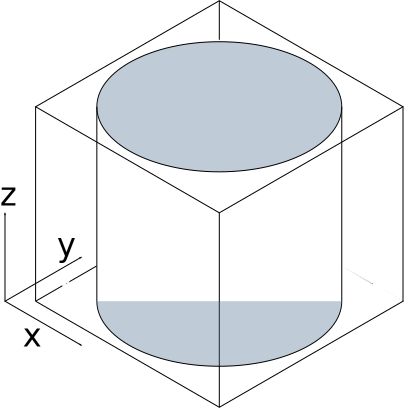
\includegraphics{gfx/cone/cylinder/cylinder.pdf}\label{fig:cone:cyl}
  \caption{blabla}

  \includegraphics{gfx/cone/cylinder/cyl_vz.pdf}\label{fig:cone:cyl_time}
  \caption{blabla}
\end{figure}
\newpage

-behaviour known theorie
- paper kurz erklären symetrie warum fehlen bestimmte moden ? ?

As a first system we want to investigate the

- erstes test system cylinnder\\
- expectation

- verglein von den bedien implementierungen\\
- first test omega = 1.2 ...\\
- diskussion rand compare to tcflow \\
- test serie verschiede methoden\\
- spektrum dargesstel\\
- evtl raytracer  comparison
- heliziätte dargstellt\\
- results diskussion ip kaputt heli 0 etc \\
\subsection{Numerical Viscosity}

\newpage

\section{Simulation of a Librating Cone}

In this section we will discuss the different numerical simulations, which has been performed
with a librating cone. We begin with the comparison to the experiment performed by \citep{Beardsley1970}.
As a next step we analyse the physical behaviour when performing the transition from a cylinder
to a cone and finally  we will investigate the influence of different offsets on top of the cone.
All simulations performed in this section use the introduced setup with different geometric parameters.
As a IBM we choose the direct forcing  method of second order.

-as a convention we refer to frustom cone etc

\subsection{Simulation of the Experiment}

The setup for this simulation is oriented on the experimental setup given by \citep{Beardsley1970}, which
we disussed in section ().
In the first part of the experiment a plexiglass cylinder of height $H=\SI{19.95}{\centi\meter}$ and a radius of
$r=\SI{19.95}{\centi\meter}$ was used. The apex half angle was set to $24^{\circ}3.7^{\prime}$ degree,
which relates to our setup with $\alpha=65^{\circ}56.3^{\prime}$
For the rotation rate a frequency of $\omega =\SI{6.28}{\radian\per\second}$ was chosen.
As a fluid, water was used, the resulting viscosity,given by \citep{tipler2003}, is $\nu = \SI{1.0}{\milli\pascal\second}$.
The resulting Ekman number is given by

\begin{align}
    \Ekman = \frac{\nu}{\omega r H^2} \approx 7.72\cdot 10^{-6}
\end{align}

In the second part of the experiment the apex of the cone was replaced by a frustum through the
insertion of a bottom plate at the position $z/H = 0.261$.
For the simulation we choose an Ekman number of $\Ekman =  10^{-4}$, since a simulation of higher ekman numbers is
diffcult to realise due to the computational effort.
Furthermore we set $\alpha = \arccos(1/2) = 60^{\circ}$, $H=1$ and $r=0.5$.\\
This means that for $\omega=1$, the propagation of an inertial wave package is parallel to the slope of the cone.
For the offset on top of the cone, we obtain the condition

\begin{align}
    o = H - h_c =  1 - r\tan{\alpha} \approx 0.134
\end{align}

The simulation has two setups in analogy to the experiment.For the second part the bottom plate is set to $h_b=0.25$.
A series of simulations of these systems where performed, with the parameters

\begin{center}
\vspace*{0.7ex}
\begin{tabular}{c|c|c|c|c|c|c }
%\begin{tabular}{p{0.1\linewidth}| p{0.1\linewidth}| p{0.1\linewidth}|  p{0.1\linewidth}| p{0.1\linewidth}| p{0.1\linewidth} }
$ \leftarrow  \omega \rightarrow $ & $\Delta t$ & $\Delta x$ & $c^2$ & \Ekman  & $l_x, l_y, l_z$ & $T_{end}$\\
\hline
$[0.2,\; 2], \Delta w = \nicefrac{1}{10}$ & $10^{-5}$ & $\nicefrac{1}{128}$ & 500 & $10^{-4}$  & (\{1, 0.75\}, 1, 1) & 100\\
\end{tabular}
\vspace*{0.7ex}
\end{center}

\clearpage
%\begin{figure}[!tp]
%  \begin{minipage}[c]{0.6\textwidth}
%      \includegraphics{gfx/cone/experiment/contour.pdf}\label{fig:mask_vp}
%  \end{minipage}\hfill
%  \begin{minipage}[c]{0.3\textwidth}
%  \caption{Stability regions for $\Omega_s$ for different Runge-Kutta methodsi
%    Stability regions for $\Omega_s$ for different Runge-Kutta methodsi
%  }
%  \label{fig:num_rkstab}
%  \end{minipage}
%\end{figure}
%
%\begin{figure}[!tp]
%  \begin{minipage}[c]{0.3\textwidth}
%  \caption{Stability regions for $\Omega_s$ for different Runge-Kutta methods
%  Stability regions for $\Omega_s$ for different Runge-Kutta methodsi
%  }
%  \label{fig:num_rkstab}
%  \end{minipage}
%  \hfill
%  \begin{minipage}[c]{0.6\textwidth}
%      \includegraphics{gfx/cone/experiment/error.pdf}\label{fig:mask_vp}
%  \end{minipage}
%\end{figure}

\begin{figure}[!bp]
  \centering
  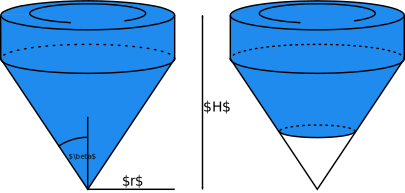
\includegraphics{gfx/cone/experiment/experiment.pdf}
  \caption{Amplitude $A\left(\left<v^2_z\right>_V\right)$ as a function of the libration frequency $\omega$,
            for a cone and a frustum.  \label{fig:cone_expseries} }
\end{figure}

\subsubsection{Results \& Discussion}
\label{cone:exp}

The results of the simulations are shown in figure \ref{fig:cone_expseries}.
For both cases, the frustum and the cone, we can observe an increase in $A\left(\left<v^2_z\right>_V\right)$
from $\approx 2\cdot10^{-4}$ at $\omega=0$ to  $\approx 3.4\cdot10^{-4}$ for the frustum and $\approx 4\cdot10^{-4}$ for the cone,  at $\omega=1$.
From here one the Amplitude decreases to $\approx 5\cdot10^{-5}$ at $\omega=2$.\\
A difference between the two setups can be observed in the surrounding area of $\omega=1$.
For the cone the increase of the amplitude is interrupted at $\omega=0.6$, a minimum can be observed at $\omega=0.8$, followed by
a peak at $\omega=1$. For the frustum the minium is not directly visible but it can be noted that the
amplitude does not increase as much at $\omega=0.7$, as for lower frequencies.\\
The maximum occurs at $\omega=0.9$, in comparison to the cone we see an increase in the amplitude of $\approx 5\cdot10^{-5}$.
However, it has to be considered, that due do the stepwidth of $\Delta \omega = 0.1$, the exact position of the maxima is
not apparent.\\
One possible assumption, regarding the position of the maximum with respect to the frequency, is that
the expansion of the frustum with a tip  results in a shift to lower frequencies.
The left shift in the decrease for $\omega > 1$ furthermore supports this idea.\\
Overall it appears that the spectrum can be divided into two domains $\Omega_1~=~\{0\leq\omega<1$\} and $\Omega_2~=~\{1\leq\omega\leq2\}$.
This result is not unexpected, since we choose the slope $\alpha$ of the cone such that for $\omega=1$, it is parallel
do the group velocity $\vec{c}_{g}$.
For $\omega\in\Omega_1$ the results for both setups are similar, since in this domain, the cone tip does not act as an attractor.
An inertial wave propagates the top, after a reflection on the side of the cone.
Hence, for both setups we obtain a similar spectrum.
The differences occur when $\omega$ is reaching the critical slope, in this scenario an inertial wave propating from the
top edges, travereses directly into the apex of the cone, or is reflected slightly at he bottom plate of the frustum.
As a results we see the increase in the amplitude.
For $\omega\in \Omega_2$ we would expect further reflections for the frustum, however the similar
decay of the amplitude refutes this assumption.\\
The results of the simulation do not match with the ones of the experiment we discussed in section ().
A possible explanation we want to propose here, is the use of a different Ekman number, which is of order $10^{-4}$ in contrast
to the one of the experiment of $10^{-5}$.
As a consequence the width of an inertial wave packet, given by $\propto \Ekman^{1/3} \approx 2\cdot10^{-2}$ (see \citep{} or section...),
is around twice the size as in the experiment. We assume that as a results a wave reflecting on the bottom of the frustum
is strongly damped due to wall friction.
DISCUSS T:\\
damping  could be propt $\Ekman \vec{K}$.

\subsection{Transition to from a Cylinder to a Cone}

We now want to further investigate the results from the previous simulation.
The assumption was made, that the inserted bottom plate is to narrow to support an efficient reflection
of inertial waves, due to frictional losses at the bottom of the cone. Thus, the next objective would be to
test the influence of different gap radii $r$.\\
We propose a setting where we begin with the possible largest bottom gap, which is $r=0.5$.
As a next step we iteratively decrease the size of the gap by $\Delta r = 0.125$ until $r=0$ is reached.
An alternative approach to this woudld be to change the offset from the bottom of the cone, which would result in a constant
slope but different heights of the simulation domain.
The influence on the simulation domain is shown in figure ()(b).
For $r=0.5$ the domain is given by a cylinder, which than transforms into a cone with a frustum and finally with an apex for $r=0$.
The main simulation parameters are given by

\begin{center}
\vspace*{0.7ex}
\begin{tabular}{c|c|c|c|c|c|c|c }
%\begin{tabular}{p{0.1\linewidth}| p{0.1\linewidth}| p{0.1\linewidth}|  p{0.1\linewidth}| p{0.1\linewidth}| p{0.1\linewidth} }
$\leftarrow r \rightarrow$ & $ \leftarrow  \omega \rightarrow $ & $\Delta t$ & $\Delta x$ & $c^2$ & \Ekman  & $l_x, l_y, l_z$ & $T_{end}$\\
\hline
$[0,\; 0.5], \Delta r =0.125$ & $[0.2,\; 2], \Delta w = \nicefrac{1}{10}$ & $10^{-5}$ & $\nicefrac{1}{128}$ & 500 & $10^{-4}$  & (1, 1, 1) & 100\\
\end{tabular}
\vspace*{0.7ex}
\end{center}
%
%\subsubsection{Results \& Discussion}
%\begin{figure}[!bp]
%      \begin{minipage}[c]{0.4\textwidth}
%      \centering
%        \resizebox{0.8\textwidth}{!}{
%       \import{gfx/cone/transition//}{attractor.pdf_tex}
%      }
%      \end{minipage}\hfill
%  \begin{minipage}[c]{0.6\textwidth}
%      \caption{
%          Wave attractor in a cylinder $\left(\text{\colorbox{green}{\textcolor{green}{o}}{\null}}\right)$
%          and shifted\\ attractor $\left(\text{\colorbox{red}{\textcolor{red}{o}}{\null}}\right)$
%          for $r<0.5$. To maintain the same attractor the point of reflection has to be at the same height $h_r$.
%      }
%      \label{cone:theorie}
%      \end{minipage}\hfill
%\end{figure}



\subsubsection{Results \& Discussion}

The results of the simulations are shown in figure \ref{fig:cone:transition}.
For $r=0$ we can see the inertial modes of a librating cylinder, which is in accordance
to the results we discussed in section \ref{cone:sec:lib_cylinder}.
With an decrease of the radius we can observe a change in the position and amplitude of the
inertial modes. We want to exemplarly discuss this pattern for the (2, 2) mode at $\omega=1.3$, where it is the best visible.
For all other modes the transition results in a similar behvavior.\\

\begin{figure}[!pt]
  \centering
  \includegraphics{gfx/cone/transition/transition.pdf}
  \caption{\label{fig:cone:transition}
    Simulation of
  }
\end{figure}

The decrease of the radius leads to a shift to lower frequencies of the (2, 2) mode,
from $r=0$ to $r=0.375$ it is of the order $\Delta \omega=0.1$.
Furthermore we can see, that during the transition a damping of the mode occurs.
For $r=0.5$ the amplitude is of order $\approx8.9\cdot10^{-3}$, for $r=0.375$ it is
$\approx8.9\cdot10^{-3}$ and for $r=0.25$ we obtain $\approx3.8\cdot10^{-3}$.\\
Whereas the first decrease of the radius does not significantly affect the amplitude,
the second decrease leads to a strong damping to less than half of the original size.
With a further decrease in $r$, the (2, 2) mode is annihilated.
\footnote{ for the possible (1, 2) mode we still can observe a slight increase of the amplitude at $r=1.4$}
One possible explanation for the shift can be given
by having a look at the inertial mode structure, for different radii as shown in figure \ref{fig:cone:phase}.\\
For $r=0.5$ we have an inertial mode, which is symmetric to the plane $h/2$.
In this plane, the waves excited from the bottom and top of the cylinder, annihilate each other and form a wave node.
An decrease of radius breaks the axial symetrie of the inertial mode.
As a result only a distorted version of the mode can exist, where the center of the wave node
is given by the intersection of the diagonals from the top to the bottom edges of the frustum.
In order to obtain the new shape it is necessary to increase the propagation angle $\Theta$,
which is equivalent to lowering the libration frequency.
We can furthermore say that for $r \rightarrow 0$, the center given by

\begin{align}
c  = r \frac{h}{r+\nicefrac{l_x}{2}}
\end{align}

converges against zero, hence a mode cannot exist in this state.
Beside the changes of the inertial modes it can be noted, that simultaneously to the decrease of the radius,
a lift of the amplitudes at lower frequencies occurs.
The vertical lines in figure \ref{fig:cone:transition} are set to the position $\omega=\Theta$.
The area $\omega<\Theta$ can again be associated with the frequency domain, where the wave propagation angle $\Theta$ is larger than
the  slope of the cone $\alpha$ and waves propgate to the top, up on reflection on the slope.
For $r=0$ we have the indentical setup to the simulation in section \ref{cone:exp}.

\begin{figure}[!pt]
  \centering
  \includegraphics{gfx/cone/transition/phase.pdf}
  \caption{\label{fig:cone:phase}
    Simulation of
  }
\end{figure}

\clearpage

\subsection{Librating Cone with different Offsets at the Top}

Finally we want to improve the setup we introduced in section \ref{exp},
by considering the insights we gained from the previous simulations.
As we pointed out, the radius at the bottom of the frustum has a strong influence on
the reflection of inertial waves, due to the larger Ekman number we use in comparsion to the experiment.
Hence, we insert the bottom plate in the cone at a height of $h_b=0.375$, the resulting radius is
$r \approx 0.22$. The total height is than given by $h=0.625$,
and the slope is unchanged.
Secondly we want to adress the influence of the offset on top of the cone,
which has been left out from any discussion so far.
We assume that this offset has an strong influence for the intervall $\Theta<\alpha$,
where wave reflection to the top occurs.
In the case where $o=0$, the corners of the cone would act as an attractor, as pointed out in figure \ref{cone:img_finalattractor}.

\begin{figure}[!bp]
      \centering
        \resizebox{0.7\textwidth}{!}{
       \import{gfx/cone//}{comparison.pdf_tex}
      }
      \caption{
          Wave reflection for $o>0$ in the upper edges of the cone (left) and
          an attractor for $o=0$ (right), in the upper edges of the cone.
      \label{cone:img_finalattractor}
      }
\end{figure}

For small gap sizes it also applies that a inertial wave will be damped.
Therefore, in this simulation we will add an additional offset to the default of $\tan(\pi/3)/2$
varying in the range of $h_+ = [0, 1]$ with a stepsize of $\Delta h_+ = \nicefrac{1}{5}$.
The main simulation parameters are given by

\begin{center}
\vspace*{0.7ex}
\begin{tabular}{c|c|c|c|c|c|c|c }
%\begin{tabular}{p{0.1\linewidth}| p{0.1\linewidth}| p{0.1\linewidth}|  p{0.1\linewidth}| p{0.1\linewidth}| p{0.1\linewidth} }
$\leftarrow r \rightarrow$ & $ \leftarrow  \omega \rightarrow $ & $\Delta t$ & $\Delta x$ & $c^2$ & \Ekman  & $l_x, l_y, l_z$ & $T_{end}$\\
\hline
$[0,\; 0.5], \Delta r =0.125$ & $[0.2,\; 2], \Delta w = \nicefrac{1}{10}$ & $10^{-5}$ & $\nicefrac{1}{128}$ & 500 & $10^{-4}$  & (1, 1, 1) & 100\\
\end{tabular}
\vspace*{0.7ex}
\end{center}

Furthermore we will compute the normalized helicity of the system given by

\begin{align}
H(t) = \frac{\int_V \dif V \vec{v} (\nabla \times \vec{v})}{\int_V \dif V |\vec{v}||\nabla \times \vec{v}|}
 = \frac{\sum_{i,j,k=0}^{N_x, N_y, N_z} \vec{v}_{i,j,k} (\nabla \times \vec{v}_{i, j, k})}
 {\sum_{i,j,k=0}^{N_x, N_y, N_z}|\vec{v}_{i,j,k}|| \nabla \times \vec{v}_{i, j, k}|}
\end{align}

in the accelerated frame of reference and also for the inertial system with an additional offset in the velocity
given by $\vec{u} = \vec{u}|_{\text{rot.}} + \Omega(t) \times \vec{r}$.
\\


The discretization of the rotation operator is using a central difference of second order.
As a next step we want to furthermore analyze the decay of inertial waves for the different offsets.
For this reason we use the end state from the previous simulations and set
the libration amplitude to zero.
Furthermore we change the end time of the previous simulations by

\begin{align}
    T = \frac{1}{\Delta t} \text{floor}\left(\text{T}_{\text{end}}\frac{\omega}{2\pi}\right)\frac{2\pi}{\omega} + \frac{2\pi}{\omega}
\end{align}

to make sure that for all frequencies the librating force drops out when crossing zero.
The main simulation parameters are given by

\begin{center}
\vspace*{0.7ex}
\begin{tabular}{c|c|c|c|c|c|c|c }
%\begin{tabular}{p{0.1\linewidth}| p{0.1\linewidth}| p{0.1\linewidth}|  p{0.1\linewidth}| p{0.1\linewidth}| p{0.1\linewidth} }
$\leftarrow r \rightarrow$ & $ \leftarrow  \omega \rightarrow $ & $\Delta t$ & $\Delta x$ & $c^2$ & \Ekman  & $l_x, l_y, l_z$ & $T_{end}$\\
\hline
$[0,\; 0.5], \Delta r =0.125$ & $[0.2,\; 2], \Delta w = \nicefrac{1}{10}$ & $10^{-5}$ & $\nicefrac{1}{128}$ & 500 & $10^{-4}$  & (1, 1, 1) & 100\\
\end{tabular}
\vspace*{0.7ex}
\end{center}

As a last step we will repeat a part of the simulations for an Ekman number of $\Ekman = 10^{-3}$

\subsection{Results}
\subsubsection{Simulation with Different Offsets}


-comper cone to frustum
-offset propt to peak shift to left
-amplitude

-plot peak shift
-plot amplitude shift

-discuss plot


\subsubsection{Simulation with no Libration}

\clearpage


\begin{figure}[!pt]
  \centering
  \includegraphics{gfx/cone/final/transition.pdf}
  \caption{\label{fig:cone:finaltransition}
    Simulation of Discussion}
\end{figure}


-description\\
-verfahren und serie\\
-diskussion oberer rand\\
-eigenschaften und influence oberer rand \\


Finally
-nun cone mit und ohne spitze
-teste den einfluss der oberen kante blablabla
-serien vergleich diskussion\
-helizität diskussion\\

In order to test
As a first test

\subsection{Discussion}


\section{Summary}
freeslip besser





\chapter{Conclusions and Outlook}

In the first part of this thesis different Immersed Boundary methods were
implemented and successfully tested with a GPU based algorithm.
The validation showed that these methods give good results for No-Slip boundaries,
the use with velocities different from zero at the boundaries tends to be problematic.
One concern of the validation is that only steady-state flows were used as test cases.
This approach is justified since the local error created trough approximations of the boundaries
has a larger influence on the global error .
However, for further validations unsteady flows could be of interest.
The validation results of the interpolation method showed by far the smallest numerical error.
Unfortunately this method became numerically unstable for the simulations of the librating cylinder and cone.
For possible future applications it would be important to find the origin of this instability.

The Immersed boundary methods introduced in this thesis were used to satisfy No-Slip boundaries, however,
in many scenarios it is necessary to use No-Flux and Free-Slip boundaries, one example is the Rayleigh-B\'{e}nard system.
In this system a fluid in a cubic or cylindric container is heated from below and cooled from above, the resulting
heat transport is purely diffusive for small temperature gradients and
becomes convective for large temperature gradients above a critical instability.
For experiments and numerical simulations of this system adiabatic side walls are used \citep{Lulff2011}.

A simple extension of the Volume-Penalization method was performed in \citep{Lulff2011}.
To enable No-Flux walls for the temperature, a inhomogenous thermal diffusivity $\kappa (x, y, z)$ was introduced.
By setting $\kappa(x, y, z) \ll 1$ in the boundary domain gives a decent approximation of No-Flux walls \citep{Lulff2011}.
An further improved version of the Volume-Penalization method for No-Flux walls can be found in \citep{Brown-Dymkoski2014}.
Here, the No-Flux boundary are obtained by introducing a forcing term of the form

\begin{align}
    \vec{f}  = -\frac{H}{\nu_c}\left( n_k\pdn[v]{x_k} - q(\vec{r}, t) \right)
\end{align}

where $\nu_c$ is a regulation parameter, and $\vec{n}$ the normal and $\vec{q}$  the desired flux through the boundary.
With this implementation the temperature flux is forced to zero in normal direction.

%TODO
Both of these methods were implemented and a first test simulation verfied the numerically stability.
However, a proper validation need to be carried out in the future.
An implementation of Immersed boundary methods for No-Flux walls would give the possibility
to simulate this flow for example in a cylinder.
%TODO

The use of Free-Slip boundaries could reduce the numerical oscillations in the simulations of the librating cone.
These oscillations are a results of the large Peclet number of the system and are generated
close to the boundaries where the velocity gradients are the largest.

In simulations of precession driven dynamos in a cube with small Ekman numbers ($\propto 10^{-5}$),
no oscillations occur when using Free-Slip boudaries \footnote{Private communication O.Goepfert}.

A first implementation of Free-Slip boundaries was performed
by inserting diagonal walls into the fluid domain which overlap with grid points.
%The idea of this approach was to mirror the
On these walls the Free-Slip condition can simply be applied just like in the basic GPU algorithm,
using the the mirroring method introduced in Sec. \ref{sec:cuda_boundaries}.
However a first test of this implemenation became numerically unstable which is not understood so far.
It would be desirable to obtain a stable Free-Slip implementation for future applications.

There are some proposals regarding the basic implementation of the algorithm on the GPU.
Numerical oscillations in the density could be a concern for future simulations.
This problem seems to be quiet common for numerical computations involving first order derivates in CFD problems.
A common approach to avoid this is the use of a staggered grid, where the velocities
are stored on the cell faces and the scalar fields in the cell center.

Alternatively, different methods exists for pressure-based solvers where the pressure is interpolated to the cell faces.
One popular method in partical is the Rhie-Chow interpolaton \citep{uiae},
different improvements of this method can be found in literature \citep{uiae} that could be used for a future implementation.

It could be of further interest to implement an unstuctured cartesian grid into the GPU algorithm.
This is a really difficult task which would in return bring some drastically improvements.
The error of the Immersed Boundary methods could be decreased by using a higher resolved grid in the vicinity to the boundary.
This would furthermore  improve the resolution of boundary layers  and reduce the oscillations resulting from the use of high Peclet numbers.

In the second part of this thesis Immersed Boundary methods were applied to different setups of a librating cylinder, cone and a frustum.
The results of these simulations are in agremeent with theoretical
predictions \citep{Greenspan1969} and experimental results \cite{Beardsley1970}.
An experimental study of these systems is in discussion as a possible future research project.
A possible experimental setup is already in development.
It contains of a rotating table, which can be controlled over a serial interface to enable a different angular velocities and acceleration rates.
A camera module is integrated into the rotating frame and could be used for the computation
of the velocity files with a PIV\footnote{Particle Image Velocimetry  - see for example \citep{aie} }
method.
With this setup it would be possible to validate the numerical results of this thesis.
Futhermore different excitation mechanism of inertial waves could be studied.
Of particular intest wolud be the study of turbulent decay in the apex of the cone.
A similar numerical study has been performed in \citep{} where a oscillating grid
was used to induction of turblent flows.





\newpage
\thispagestyle{empty}
\mbox{}

\begin{appendices}
\chapter{Additional Figures}

\section{Poiseuille Flow}
\begin{figure}[!h]
    \centering
    \includegraphics{gfx/immersed_boundary/poiseuille_flow/3_df/relative_l2error.pdf}
    \caption{Relative $l_2$-error for the DF-FD2 and DF-FD4 method.}
    \label{fig:vali_pflow_3gc}
\end{figure}

\clearpage

\section{Hagen-Poiseuille Flow}

\begin{figure}[!h]
  \centering
  \includegraphics{gfx/immersed_boundary/hpflow/long/rho.pdf}
  \caption{Densitiy oscillations for different Immersed Boundary methods with the use of FD4. The IP+DF FD4 method is not stable.}
    \label{fig:hpflow_allgc_theo}
\end{figure}
\clearpage

\section{Taylor-Couette Flow}

\begin{figure}[!h]
  \includegraphics{gfx/immersed_boundary/tcflow/long/vz_profiles_o4.pdf}
  \caption{\label{tcflow:results_vprofiles_o4}
    Substraction of the numerial velocity profile from the theoretical
        for all FD4 methods.}
\end{figure}
\clearpage

\begin{figure}[!h]
  \includegraphics{gfx/immersed_boundary/tcflow/long/rho_o2.pdf}
  \caption{Density oscillations for different Immersed Boundary methods of the FD2 methods.}
    \label{tcflow:results_rho_profiles_o2}
\end{figure}
\clearpage

\chapter{Source Code}

%\begin{lstlisting}[caption='RK-Stability Computation']
\section{Runge-Kutta stability computation}
\begin{python}[label={lst:appendix_rkstab}]
import matplotlib.pyplot as plt
import numpy as np
from math import factorial as fac
from scipy import interpolate

def radial_sort(x, y):
    """Sort line by angle from center (-1, 0)"""
    angle = np.arctan2(y, x + 1.)
    idx = angle.argsort()
    x, y = x[idx], y[idx]
    # Split at opening in line
    dx = np.diff(np.append(x, x[-1]))
    dy = np.diff(np.append(y, y[-1]))
    max_gap = np.abs(np.hypot(dx, dy)).argmax() + 1
    x = np.append(x[max_gap:], x[:max_gap])
    y = np.append(y[max_gap:], y[:max_gap])
    return x, y

def main():
    f, ax = style.newfig(0.8)
    x = np.linspace(-4, 4, 1500)
    X, Y = np.meshgrid(x, x)
    C = X + 1j*Y

    for i in range(1,6)[::-1]:
        b = np.zeros_like(C)
        for j in range(0,i):
            b += C**j/fac(j)
        out = np.where(np.diff((np.abs(b)<=1).astype('float')) != 0)
        pts = np.column_stack((X[out], Y[out]))
        x, y = pts[:, 0], pts[:, 1]
        try:
            x, y = radial_sort_line(x,y)
            x = np.append(x, x[0])
            y = np.append(y, y[0])

            tck, u = interpolate.splprep([x, y], s=0)
            unew = np.linspace(0, 1.0, 100)
            out = interpolate.splev(unew, tck)
            plt.plot(out[1], out[0])
        except:
            print 'Error for %i' % i
    plt.show()

if __name__=='__main__':
    main()

\end{python}
%#\end{lstlisting}
\clearpage


\chapter{Python Simulation API}

\section{Introduction}

In this chapter a brief overview will be given to the high object oriented simulation API which
was written in the context of this thesis, with the python programming language.
The purpose of the library in general is to simplify the execution of simulations but furthermore
includes the possibility to analyse the results and use visualization techniques to study the overall
behavior of the simulations during runtime.
At first some of the  different API classes and objects will be introduced,
followed by a small application in form of a grid convergence study.

\section{Parameter File}

The Parameter file contains every flag and parameter which is used during the runtime of the simulation.
During compile time all parameters are converted into a specific set of C-macros which are then compiled
into the CUDA code. As a file format the open-standard format \textbf{Json} \footnote{Javascript Object Notation} is used.
An example of a Parameter file is shown in Listing \ref{lst_json}, it contains of two sections:

\begin{description}
\item[Conditions] Flags which are set to a constant value during runtime mostly zero or one. For example the boundary conditions and
                  interpolation methods. Not all flags have to be set for a simulation.
\item[Parameters] This set defines all parameters which are used  for a simulation. In contrast to the conditions each
                  parameter has to be defined in order to enable a proper execution.
\end{description}

\begin{minipage}{\linewidth}
\begin{lstlisting}[language=json, caption={'Example of a "parameter.json" file.}, label={lst_json} ]
{
    "conditions": {
        "all_periodic" :1  //periodioc boundaries in all directions
    },
    "parameters": {
        "BLOCKSIZE": 8,                //Defaultl GPU blocksize
        "STEPMAX": 200000,             //Number of timesteps
        "IC_NAME": "\"c2_1000\"",      // Initial condition files (not in use anymore)
        "RAYLEIGH":0,                  // Rayleigh number, not used in this thesis
        "DELTA_T": 0.0001,             // Time step
        "SOUND_SPEED_SQUARED": 400,    // Speed of sound squared
        "PRANDTL": 0.01,               // Prandtl number, not used in this thesis
        "GPU_ID": 2,                   // GPU id, there are up to 8 gpus in one system
        "EKMAN": 0.0001,               // Ekman number
        "NX": 64,                      // Resolution in x-direction
        "NY": 64,                      // Resolution in y-direction
        "NZ": 64,                      // Resolution in z-direction
        "LX": 1.0,                     // Length in x-direction
        "LX": 1.0,                     // Length in y-direction
        "LZ": 1.0,                     // Length in z-direction
        "LZ": 1.0,
        "RUN_NAME": "\"c2_1000\"",     //Name of .ekin output files
        "NUM_GPU": 1,                  //Number of GPUs used for the computation
        "SAMPLING_RATE": 5000,         //Number of samplings for data analysis
        "NX_D": "NX/NUM_GPU",          //NX for one GPU with threadings
        "NU": 0.0001,                  //Damping force
        "PM": 1,                       //Magnetic Prandtl number (not used)
        "KAPPA": 0.0001                //Thermal diffusivity (not used)
    }
}
\end{lstlisting}
\end{minipage}

\section{Generator Class}

The generator class is responsible for the generation of all initial data.
This means the initial conditions for all variables i.e. velocity, temperature
and the computation of interpolation and domain masks which are necessary for the different
IB methods.\\
During the execution of a simulation all precomputed arrays are stored within a
HDF5-File format, which is optimized for the storage and structuring of large amounts of data.
Furthermore, the format simplifies the data exchange between the python API and the CUDA program.

For the generation of data a generator object has to be initialized with a generator function,
there are currently implemented two different types of these functions.

\begin{description}
\item[Initial  Conditions] These functions simply generate the initial conditions for a certain flow problem, for example the Taylor-Couette
                            flow or a simple cylindric domain. The definition of the functions can be found in \textbf{pycurb.ic}.
\item[Testcase] The test case functions extend the initial conditions the possibility to add certain forcing parameters into the time step
                for example a pressure gradient is necessary for the Poiseuille flow test case described in Sec. \ref{vali:sec_lpflow_setup}
                All defined functions can be found in \textbf{pycurb.testcase}.
\end{description}


\begin{python} [caption='Generator class usage', label={gen_class_usage}]
import pycurb as pc #import the simulation API
import pycurb.testcase as tf #import test cases
import pycurb.ic as as ic    #import initial conditions

#create a generator object for hagen poiseuille flow in z direction
generator = pc.Generator.from_testcase(tf.cylinder_flow_z)
#set the default velocity profile, pressure gradient and radius
generator.add_option('SETV', True)
generator.add_option('PMAX', pmax)
generator.add_option('r', 1.)

#create a generator object for taylor couette flow
generator = pc.Generator.from_ic(ic.taylor_couette)
#set velocity, inner and outer radius
generator.add_option('SETV', True)
generator.add_option('ri', ri)
generator.add_option('ro', ro)
\end{python}

Additionally it is possible to create a generator which takes the data from an old simulation. In listing \ref{gen_class_usage} the creation of a generator object is
exemplary shown. In a first step the generator is created by using a generator function. In the next step it is possible to define certain attributes
for example the radius of a cylindric fluid domain.

\section{Simulation Class}

An instance of the simulation class is the main object of the API and
necessary to execute a simulation. For the creation of a simulation object
the initial arguments are the file path, where all simulation data will be stored
and the json-file for the parameter setting.
Following the creation of the simulation object it is possible to alter all parameters and conditions
which were previously stored in the json-file. This gives the possibility to create
simulations with different parameter settings on the fly, i.e. changing the resolution of the numerical grid
to perform a grid convergence study.
Before the execution of the CUDA code, the simulation object has to be bind to a generator object
with the \textbf{generate\_files} class function, in return the generator object will begin
with the data creation. The last step is the execution of the CUDA code which can be done with the \textbf{start\_simulation}
class function.  A minimal use case of the complete procedure is shown in listing \ref{gen_usage_nextone}.

\clearpage

\begin{python}[caption='Simulation class usage', label={gen_usage_nextone}]
import pycurb as pc
import pycurb.ic as ic

#create a generator
generator = pc.Generator.from_ic(ic.taylor_couette)
#create a simulation object
sim = pc.Simulation('data', 'parameter.json')
sim.parameter.set('NX', 128)
sim.parameter.set('NY', 128)
sim.parameter.set_condition('o2', order)
sim.generate_files(generator)
#start the simulation
sim.start_simulation()
\end{python}

\section{Usage Example}

Finally a usage example for a grid convergence study using the Simulation API is given.
The source code is shown in listing \ref{gcstudy_papi}.
In the example  a Hagen-Poiseuille flow is simulated (see Sec. \ref{vali:section_hpflow_start}).

As first step all modules from the API are imported and all relevant constants are defined, for example the
Reynolds number is set to  $Re=100$.
In the next step a  for-loop iterates over the  array which contains all resolutions for which the
simulation should be executed.

Inside the for-loop the first step is to set a unique simulation path for each resolution.
Next, a generator with the pipe-flow settings from the \textbf{pycurb.testcase} module is created
and the options for the pressure gradient, the initial velocity field and the pipe radius are set.

Finally the simulation object is created. All parameters like resolution and domain size,
the order of the finite difference scheme and the direct forcing method are set.
The last step is the execution of a simulation.\\
%The given example is build to be executed on a single machine in order to further parallize the computations on
%more than one gpu an additional python script \textbf{worker.py} was written which is not yet included in the simulation API (see Appendix A(XX)).
%To parallelize the example some small adaptions has to be made. For each resolution the simulation path has to be stored into a textfile, which
%is than opened by the python script, furthermore the execution of the simulation has to be removed from the for-loop.
%Finally we start by generating all simulation data by executing the modified version of our script. Afterwards we start
%the parallelization script for which we have to specify the file including the simulation path and the number of gpus and cuda machines we want to use.

\clearpage

\begin{python}[caption='Grid Convergence Study Example', label={gcstudy_papi}]
import pycurb as pc
import pycurb.testcase as tf
import numpy as np
import os

def main():
    #define simulation parameters
    re = 100.
    pmax, pr = 4./re,  1./re
    lx, ly, order = 2.5, 2.5, 1

    #vary N from 16 to 256 with dN=16
    res = np.linspace(16, 256., 256./16)

    for rs in res:#iterate through resolution array
        #create filepath for each simulation
        var_path = os.path.join(method,'res_%i' % rs)
        sim_path = os.path.join(os.path.dirname(__file__), "data", var_path)

        #create generator with simulation settings
        generator = pc.Generator.from_testcase(tf.cylinder_flow_z)
        generator.add_option('SETV', True)
        generator.add_option('PMAX', pmax)
        generator.add_option('r', 1.)

        #create simulation object and set parameters
        sim = pc.Simulation(sim_path, "parameter.json")
        sim.parameter.set("PRANDTL", pr)
        lz = dx*(lx/rs)
        sim.parameter.set("NX", rs)
        sim.parameter.set("NY", rs)
        sim.parameter.set("LX", lx)
        sim.parameter.set("LY", ly)
        sim.parameter.set("NZ", nz)
        sim.parameter.set("LZ", lz)
        sim.parameter.set_condition('o2', order)
        sim.parameter.set_condition('SET_ZERO', 1)
        sim.generate_files(generator)

        #execute simulation
        sim.start_simulation()

if __name__=='__main__':
    main()
\end{python}

%The script creates a thread-safe queue and a number of threads, one for each gpu per machine.
%Each thread automatically fetches a job from the queue, than logs into the assigned cuda machine
%and executes the job on the given gpu.
%For time consuming simulations also a modificated version of the script was written where one thread
%can use more than one gpu, see Appendix A(XX).

\end{appendices}

\begingroup
\sloppy
\printbibliography
\endgroup

 \chapter*{Danksagung}

\begin{otherlanguage}{ngerman}
  \thispagestyle{empty}





  \null\vfill
  \noindent
\end{otherlanguage}

\begin{otherlanguage}{ngerman}
  \clearpage\thispagestyle{empty}
  \null\vfill
  \noindent
  \begin{tabular}[t]{p{0.175\textwidth}p{0.825\textwidth-4\tabcolsep}}
    \bfseries\large Erkl\"arung&nach
    \S17(9)  der Prüfungsordnung für den
    Bachelor-Studiengang Physik und den Master-Studiengang Physik
    an der Universität Göttingen:\\[1em]
    &Hiermit erkläre ich, dass ich diese Abschlussarbeit
    selbständig verfasst habe, keine anderen als die
    angegebenen Quellen und Hilfsmittel benutzt habe und alle Stellen,
    die wörtlich oder sinngemä\ss{} aus veröffentlichten Schriften
    entnommen wurden, als solche kenntlich gemacht habe.

    Darüberhinaus erkläre ich, dass diese Abschlussarbeit nicht, auch nicht
    auszugsweise, im Rahmen einer nichtbestandenen Prüfung an dieser oder
    einer anderen Hochschule eingereicht wurde.\\[1em]
    &\begin{center}Göttingen, den \today\end{center}\\[1.5cm]
    &\begin{center} (Jonas Ruebsam)\end{center}
    %\begin{minipage}[t]{0.76\textwidth-4\tabcolsep}
    %  \@author\end{minipage}
  \end{tabular}
\end{otherlanguage}

\end{document}
